\documentclass{thesis}
% \usepackage[utf8]{inputenc}
\usepackage{csquotes}
\usepackage{enumitem}
\usepackage{blindtext}

% SIunitx formatting
% ------------------
\usepackage{siunitx}
\DeclareSIUnit\pixel{px}
\DeclareSIUnit\mag{X}
\DeclareSIUnit\NA{NA}
\DeclareSIUnit\hour{hr}
\DeclareSIUnit\molar{M}


% Biblatex formatting
% -------------------
\usepackage[
    backend=biber,
    style=numeric,
    sorting=none,
    maxcitenames=2,
    mincitenames=1,
]{biblatex}
\renewbibmacro{in:}{}  % https://tex.stackexchange.com/questions/10682/suppress-in-biblatex

% Add bibresources for biblatex
\addbibresource{chapter-1/chapter-1.bib}
\addbibresource{chapter-2/chapter-2.bib}
\addbibresource{chapter-3/chapter-3.bib}
\addbibresource{chapter-4/chapter-4.bib}
\addbibresource{chapter-5/chapter-5.bib}
\addbibresource{cppendix-A/appendix-A.bib}



% THE BEGINNING
% -------------
\begin{document}

% Some useful commands
\newcommand{\needref}{[\textbf{\textcolor{red}{*REFERENCES*}}]}

% SI formatting options
\sisetup{
    range-phrase=--,
    range-units=single,
    per-mode=symbol,
    detect-all
}

% De good stuff
% -------------
\title{Pain and suffering in The Netherlands}
\author{Ryan}{Lane}
% \date{\today}

% De even better stuff
% --------------------
% Use Roman numerals for the page numbers of the title pages and table of
% contents.
\frontmatter
% \maketitle
\begin{titlepage}

\begin{center}

% Extra whitespace at the top.
\vspace*{2\bigskipamount}

% Print the title.
{\makeatletter
\titlestyle\bfseries\LARGE\@title
\makeatother}

% Print the optional subtitle.
{\makeatletter
\ifx\@subtitle\undefined\else
    \bigskip
    \titlefont\titleshape\Large\@subtitle
\fi
\makeatother}

\end{center}

\cleardoublepage
\thispagestyle{empty}

\begin{center}

% The following lines repeat the previous page exactly.

\vspace*{2\bigskipamount}

% Print the title.
{\makeatletter
\titlestyle\bfseries\LARGE\@title
\makeatother}

% Print the optional subtitle.
{\makeatletter
\ifx\@subtitle\undefined\else
    \bigskip
    \titlefont\titleshape\Large\@subtitle
\fi
\makeatother}

% Uncomment the following lines to insert a vertically centered picture into
% the title page.
%\vfill
%\includegraphics{title}
\vfill

% Apart from the names and dates, the following text is dictated by the
% promotieregelement.

{\Large\titlefont\bfseries Proefschrift}

\bigskip
\bigskip

ter verkrijging van de graad van doctor

aan de Technische Universiteit Delft,

op gezag van de Rector Magnificus Prof.~dr.~ir.~T.H.J.J.~van der Hagen,

voorzitter van het College voor Promoties,

% in het openbaar te verdedigen op dinsdag 1 januari 2022 om 10:00 uur
in het openbaar te verdedigen op [promotiedatum en tijdstip]

\bigskip
\bigskip

door

\bigskip
\bigskip

% Print the full name of the author.
\makeatletter
{\Large\titlefont\bfseries\@firstname\ {\titleshape\@lastname}}
\makeatother

\bigskip
\bigskip

Master of Science in Applied Physics, \\
University of Oregon, Verenigde Staten van Amerika,

geboren te Pennsylvania, Verenigde Staten van Amerika.

% Extra whitespace at the bottom.
\vspace*{2\bigskipamount}

\end{center}

\clearpage
\thispagestyle{empty}

% The following line is dictated by the promotieregelement.
\noindent Dit proefschrift is goedgekeurd door de promotoren.

% % List the promotors (supervisors).
% \medskip\noindent
% \begin{tabular}{l}
%     promotor: Prof.\ dr.\ J.\ Kleiner \\
%     copromotor: Dr.\ E.C.M.\ Carroll
% \end{tabular}

\bigskip
\noindent Samenstelling promotiecommissie:

% List the committee members, starting with the Rector Magnificus and the
% promotor(s) and ending with the reserve members.
\medskip\noindent
% \begin{tabular}{p{3cm}l}
\begin{tabular}{p{4cm}l}
    Rector Magnificus, & voorzitter \\
    Dr.\ ir.\ J.P.\ Hoogenboom, & Technische Universiteit Delft, promotor \\
    Dr.\ E.C.M.\ Carroll, & Technische Universiteit Delft, copromotor \\

    \medskip
    % \mbox{\emph{Onafhankelijke leden:}} & \\

    % Prof.\ dr.\ A.\ Jansen & Technische Universiteit Delft \\
    % % Special case, only for very long names
    % \mbox{Prof.\ dr.\ ir.\ A.B.C.D.\ van de Lange-Achternaam} & \\
    %   & Technische Universiteit Delft \\
    % Prof.\.dr.\ N.\ Nescio & Politecnico di Milano, Itali\"e \\
    % Prof.\ dr.\ ir.\ J.\ Doe, & Technische Universiteit Delft, reservelid \\

    % \medskip
    % \mbox{\emph{Overige leden:}} & \\
    % Prof.\ dr.\ ir.\ J.\ de Wit, & Technische Universiteit Delft \\
    % Dr.\ ir.\ Q.\ de Zwart, & Technische Universiteit Eindhoven \\
\end{tabular}

% Include the following disclaimer for committee members who have contributed
% to this dissertation. Its formulation is again dictated by the
% promotieregelement.
% \medskip
% \noindent Prof.\ dr.\ ir.\ J.\ de Wit heeft in belangrijke mate aan de totstandkoming van het proefschrift bijgedragen.

% Here you can include the logos of any institute that contributed financially
% to this dissertation.
\vfill
\begin{center}
    
\includegraphics[height=2.7cm]{title/logos/logos_v1.pdf}
\end{center}
\vfill

\noindent
\begin{tabular}{@{}p{0.2\textwidth}@{}p{0.8\textwidth}}
    \textit{Keywords:} & \ldots \\[\medskipamount]
    \textit{Printed by:} & Johannes Gutenberg \\[\medskipamount]
    \textit{Front \& Back:} & Beautiful cover art that captures the entire content of this thesis in a single illustration. \\[\medskipamount]
    \textit{Funding:} & This project was financially supported by the Building Blocks of Life (BBoL) program of the Netherlands Organization for Scientific Research (NWO), with cash and in-kind contributions from Delmic B.V. and Genentech.
\end{tabular}

\vspace{4\bigskipamount}

\noindent Copyright \textcopyright\ 2022 by R.~Lane


\medskip
\noindent ISBN 000-00-0000-000-0

\medskip
\noindent An electronic version of this dissertation is available at \\
\url{http://repository.tudelft.nl/}.

\end{titlepage}

\section{Propositions}

\begin{enumerate}
    \item Researchers doing SEM-based backscattered electron imaging of biological tissue without the use of a negative potential bias are wasting time. \\
    \textit{This proposition pertains to this dissertation.}
    \item Integrated array tomography is the most viable solution for acquiring large-scale correlative light and electron microscopy datasets with sub-micron registration precision. \\
    \textit{This proposition pertains to this dissertation.}
    \item By mitigating nonspecific labeling artefacts and correcting for registration errors, neural networks are capable of providing higher quality fluorescence information than fluorescence microscopes. \\
    \textit{This proposition pertains to this dissertation.}
    \item The future of correlative light and electron microscopy relies on improved protocols for sample preparation rather than instrumentation. \\
    \textit{This proposition pertains to this dissertation.}
    \item The next revolution in dense reconstruction of biological specimen will come from X-ray nano-tomography.
    \item A civilization is more likely to conquer its neighbor if it began food production first.
    \item The best way to ensure the survival of our planet is for all humans not working on an asteroid-detonation strategy to die.
    \item If intelligent lifeforms existed elsewhere in our galaxy, we would be aware of them by now.
    \item By manufacturing women's clothing with impractical or nonexistent pockets, the fashion industry has exploited women into the purchasing of hand bags.
    \item The Technical University of Delft should not tout its ``green" credentials whilst hiding the glass recycling in the basement of Building 22.
    \item Art is not open to interpretation; it means precisely what the artist meant it to and nothing more.
    \item The key factor in the success of a city is a diversified labor market.
\end{enumerate}

\tableofcontents

% De bestest stuff
% ----------------
% Use Arabic numerals for the page numbers of the chapters.
\mainmatter
\chapter{Introduction}
\label{chap:1}

% Sections
\section{Introduction}
\label{sec:4.1_intro}

Electron microscopy (EM) has transformed the way in which biologists understand intra- and inter-cellular systems. Due to the lack of inherent biological specificity, however, interpretation of EM datasets typically requires tedious expert analysis and annotation. For this reason, fluorescence microscopy (FM) is often used in conjunction with EM, complementing structural data with targeted biological labels. Fluorescent labelling, however, comes with several drawbacks. Sample preparation protocols are often laborious, involve genetic modifications, and are potentially damaging to the sample \cite{christiansen2018silico, schnell2012immunolabeling}. Protocols must also be adapted to limit concentrations of heavy metal staining if intermediate processing of the sample is to be avoided \cite{kuipers2015scanning, lane2021optimization}. Fluorescent labelling is also susceptible to bleedthrough when multiple fluorophores are expressed in a single sample as well as varying specificity---Hoechst dyes, for instance, bind to both DNA and RNA. Furthermore, registering the separate imaging modalities across large spatial extents remains a technically challenging and primarily manual task \cite{muller2014correlative, paul2017ec, russell20173d}. Correlative fluorescence and electron microscopy experiments are therefore typically limited in scope to the micron or tens of microns scale, and thus so are the regions for which biological labels can be provided \cite{de2015correlated, russell20173d}.

As recognition of organelles and other subcellular structures remains a pivotal obstacle in biological EM, we questioned whether large-scale EM datasets \cite{de2020large, dittmayer2021preparation} could be supplemented with biological labels through alternate means. To address this question, we sought to leverage recent advances in deep learning. Deep convolutional neural networks (CNN) in particular have been shown to be capable of inferring complex, non-linear relationships from image data \cite{he2016deep, januszewski2018high}. Prior work involving deep CNNs in the context of electron microscopy data has primarily been limited to applications in segmentation, denoising, and compressed sensing \cite{ede2021deep}. Semantic segmentation, the classification of pixels into discrete categories, does ultimately serve the purpose of adding biological labels to EM data. However, modern deep learning approaches require hours of tedious expert segmentation \cite{takemura2013visual, helmstaedter2013cellular, huang2014identifying, heinrich2018synaptic, liu2020automatic, spiers2021deep}. In order to perform whole-cell organelle segmentation, for instance, \SI{28}{\micro\meter^3} of training data was manually segmented; each cubic micron block required one person two weeks of manual segmentation \cite{heinrich2020automatic}.

Although relatively little attention has been paid to alternative applications in deep learning for EM data, recent work has focused on generating biological labels from other imaging modalities. \textcite{christiansen2018silico} designed a deep neural network to predict fluorescence labels from transmitted light images. \textcite{ounkomol2018label} extended the technique to generate 3D fluorescence from stacks of transmitted light microscopy data and further demonstrated the possibility of predicting immunofluorescence from EM images in order to facilitate automatic registration of fluorescence data with EM. \textcite{seifert2020deepclem} similarly developed a CNN for registering correlative datasets, releasing it as a FIJI plugin. To address the challenge of adding biological specificity to large-scale EM datasets, we thus explored the potential for a CNN to make label-free fluorescence predictions from EM (image) data.

In this work we present a deep CNN, CLEMnet, for generating fluorescence predictions on large-scale EM data of tissue and cellular samples. We demonstrate the performance of our model on thin sections of rat pancreas tissue, which have been immunolabelled with Alexa Fluor 594 and given a Hoechst counterstain, as well as Hoechst-stained sections of resin-embedded mouse breast tumor cells. Network predictions are quantitatively evaluated against corresponding true fluorescence images based on the Pearson correlation coefficient (PCC, or $\rho$) as well as by assessing human recognition of fluorescence predictions on cell nuclei. We additionally assess the network's robustness by measuring its predictive power on EM datasets acquired with a diverse range of imaging parameters. Finally, we explore the potential of correlative and predicted fluorescence signals for use as labels in segmentation experiments.


% References
\printbibliography[title={References}]
  % intro
% \chapter[Optimization of negative stage bias potential]{Optimization of negative stage bias potential for faster imaging in large-scale electron microscopy}
\label{chap:2}

% Abstract
\begin{abstract}
    Large-scale electron microscopy (EM) allows analysis of both tissues and macromolecules in a semi-automated manner, but acquisition rate forms a bottleneck. We reasoned that a negative bias potential may be used to enhance signal collection, allowing shorter dwell times and thus increasing imaging speed. Negative bias potential has previously been used to tune penetration depth in block-face imaging. However, optimization of negative bias potential for application in thin section imaging will be needed prior to routine use and application in large-scale EM. Here, we present negative bias potential optimized through a combination of simulations and empirical measurements. We find that the use of a negative bias potential generally results in improvement of image quality and signal-to-noise ratio (SNR). The extent of these improvements depends on the presence and strength of a magnetic immersion field. Maintaining other imaging conditions and aiming for the same image quality and SNR, the use of a negative stage bias can allow for a 20-fold decrease in dwell time, thus reducing the time for a week long acquisition to less than \SI{8}{\hour}. We further show that negative bias potential can be applied in an integrated correlative light electron microscopy (CLEM) application, allowing fast acquisition of a high precision overlaid LM-EM dataset. Application of negative stage bias potential will thus help to solve the current bottleneck of image acquisition of large fields of view at high resolution in large-scale microscopy.
\end{abstract}

% Published as footnote
\blfootnote{This chapter has been published as: \fullcite{lane2021optimization}.}
\clearpage


% Sections
\section{Introduction}
\label{sec:4.1_intro}

Electron microscopy (EM) has transformed the way in which biologists understand intra- and inter-cellular systems. Due to the lack of inherent biological specificity, however, interpretation of EM datasets typically requires tedious expert analysis and annotation. For this reason, fluorescence microscopy (FM) is often used in conjunction with EM, complementing structural data with targeted biological labels. Fluorescent labelling, however, comes with several drawbacks. Sample preparation protocols are often laborious, involve genetic modifications, and are potentially damaging to the sample \cite{christiansen2018silico, schnell2012immunolabeling}. Protocols must also be adapted to limit concentrations of heavy metal staining if intermediate processing of the sample is to be avoided \cite{kuipers2015scanning, lane2021optimization}. Fluorescent labelling is also susceptible to bleedthrough when multiple fluorophores are expressed in a single sample as well as varying specificity---Hoechst dyes, for instance, bind to both DNA and RNA. Furthermore, registering the separate imaging modalities across large spatial extents remains a technically challenging and primarily manual task \cite{muller2014correlative, paul2017ec, russell20173d}. Correlative fluorescence and electron microscopy experiments are therefore typically limited in scope to the micron or tens of microns scale, and thus so are the regions for which biological labels can be provided \cite{de2015correlated, russell20173d}.

As recognition of organelles and other subcellular structures remains a pivotal obstacle in biological EM, we questioned whether large-scale EM datasets \cite{de2020large, dittmayer2021preparation} could be supplemented with biological labels through alternate means. To address this question, we sought to leverage recent advances in deep learning. Deep convolutional neural networks (CNN) in particular have been shown to be capable of inferring complex, non-linear relationships from image data \cite{he2016deep, januszewski2018high}. Prior work involving deep CNNs in the context of electron microscopy data has primarily been limited to applications in segmentation, denoising, and compressed sensing \cite{ede2021deep}. Semantic segmentation, the classification of pixels into discrete categories, does ultimately serve the purpose of adding biological labels to EM data. However, modern deep learning approaches require hours of tedious expert segmentation \cite{takemura2013visual, helmstaedter2013cellular, huang2014identifying, heinrich2018synaptic, liu2020automatic, spiers2021deep}. In order to perform whole-cell organelle segmentation, for instance, \SI{28}{\micro\meter^3} of training data was manually segmented; each cubic micron block required one person two weeks of manual segmentation \cite{heinrich2020automatic}.

Although relatively little attention has been paid to alternative applications in deep learning for EM data, recent work has focused on generating biological labels from other imaging modalities. \textcite{christiansen2018silico} designed a deep neural network to predict fluorescence labels from transmitted light images. \textcite{ounkomol2018label} extended the technique to generate 3D fluorescence from stacks of transmitted light microscopy data and further demonstrated the possibility of predicting immunofluorescence from EM images in order to facilitate automatic registration of fluorescence data with EM. \textcite{seifert2020deepclem} similarly developed a CNN for registering correlative datasets, releasing it as a FIJI plugin. To address the challenge of adding biological specificity to large-scale EM datasets, we thus explored the potential for a CNN to make label-free fluorescence predictions from EM (image) data.

In this work we present a deep CNN, CLEMnet, for generating fluorescence predictions on large-scale EM data of tissue and cellular samples. We demonstrate the performance of our model on thin sections of rat pancreas tissue, which have been immunolabelled with Alexa Fluor 594 and given a Hoechst counterstain, as well as Hoechst-stained sections of resin-embedded mouse breast tumor cells. Network predictions are quantitatively evaluated against corresponding true fluorescence images based on the Pearson correlation coefficient (PCC, or $\rho$) as well as by assessing human recognition of fluorescence predictions on cell nuclei. We additionally assess the network's robustness by measuring its predictive power on EM datasets acquired with a diverse range of imaging parameters. Finally, we explore the potential of correlative and predicted fluorescence signals for use as labels in segmentation experiments.

\section{Results}
\label{sec:4.2_results}

% 4.2.1
% -----
\subsection{Network overview}
\label{sec:4results_overview}

To train a CNN to predict fluorescence intensity from EM images, we first create training datasets comprised of high-magnification EM and FM image pairs. The FM images are acquired by a fluorescence microscope integrated into the chamber of a scanning electron microscope (SEM) \cite{liv2013simultaneous, zonnevylle2013integration}. This instrumental setup allows for [sub-\SI{10}{\nano\meter} overlay precision without a reliance on fiducial markers or manual input \cite{haring2017automated}.] The lack of fiducial markers is beneficial as the network does not learn on extrinsic markers, while the lack of manual input enables the accumulation of correlative datasets to be partially automated and scalable to several GBs. A more detailed description of how integrated CLEM datasets are generated can be found in \ref{sec:2methods_acqstrat} as well as in \textcite{lane2021optimization}.

GB-sized image data is far too cumbersome for modern deep learning models to train on. The registered image data is therefore divided into small tiles which serve as input for the model (Figure \ref{fig:4.1_overview}A); the model architecture can be adjusted to support an arbitrary number of fluorescence channels. The image tiles are shuffled around to diversify the [area thereby avoiding overfitting]. A multi-layer CNN was chosen to train on due to its proven ability for recognizing structural detail in EM image data [and its performance in superhuman pattern recognition] (Figure \ref{fig:4.1_overview}B). To address the resolution mismatch between EM-FM image pairs, the model is designed with more contraction paths than expansion paths---resulting in an elongated, backwards ``J"-shape, as opposed to the more characteristic ``U". Once trained, the model is able to generate predictions of the fluorescence intensity on individual EM image tiles. Separate correlative EM-FM datasets are set aside for validating and testing the model. By stitching together the [model's output] it is possible to [render] large-scale or volume predictions of the fluorescence intensity. These can be superimposed onto the EM test dataset to generate large-scale or volume CLEM predictions (Figure \ref{fig:4.1_overview}).

% We train and test network to [list all the samples...]


% Figure 4.1 (overview)
% ---------------------
\begin{figure}[!tbh]
    \centering
    \includegraphics[width=\linewidth]{chapter-4/figures/fig1_overview_v5.pdf}
    \caption{\textbf{Overview of procedure for fluorescence intensity predictions.}
    Training data for the model consists of registered, large-scale CLEM datasets (A) comprised of high-magnification EM images and an arbitrary number of fluorescent channels. For the rat pancreas tissue shown here, the fluorescent channels consist of a Hoechst stain, targeting cell nuclei, and an AF594 immunostaining, targeting insulin granules. CLEM image data is input into an asymmetric convolutional neural network (B) which maps the EM image data to FM image data. The model is represented by an elongated, backwards J-shape as it consists of fewer upsampling layers than downsampling layers---a result of the resolution difference between the EM and FM images. Once trained, the network generates predictions from large-scale EM data (C) such that the generated predictions can be overlaid with the input EM data to generate large-scale correlative datasets of the predicted fluorescence (D).
    \textbf{[TODO: add scale bars.]}}
    \label{fig:4.1_overview}
\end{figure}



% 4.2.2
% -----
\clearpage
\subsection{Network predictions on thin tissue sections}
\label{sec:4results_pancreas}

To characterize the performance of our network, we first apply it to sections of rat pancreas tissue. The tissue is given a Hoechst stain---targeting cell nuclei---as well as immunolabelled with AF594---targeting insulin granules. The predicted fluorescence signal (green) is found to correlate well with the true fluorescence (red) (Figure \ref{fig:4.2_pancreas}). When applied to an entire islet of Langerhans, the network registers Pearson correlation coefficients (PCC) of 0.67 and 0.76 for the predicted Hoechst and AF594 signals respectively. At high magnification, the predicted signals are found to exhibit a close qualitative resemblance (Figure \ref{fig:4.2_pancreas} insets). Notably, the true Hoechst fluorescence is more heavily concentrated along the nuclear envelope, whereas the predicted Hoechst signal is relatively stronger in regions of denser chromatin. The predicted AF594 signal matches well with that of the true fluorescence with the caveat that it appears somewhat blurred, likely due to the insulin granules themselves being diffraction-limited. There are other factors that may contribute to a diminished PCC that are extraneous to the network. These include bleedthrough of one fluorescence channel into another (Supplemental Figure \ref{fig:4.S1_rois}B), errors in the EM-FM registration (Supplemental Figure \ref{fig:4.S1_rois}C), and aberrations in the true fluorescence microscopy images (Supplemental Figure \ref{fig:4.S1_rois}D). Not only do these examples help justify a reduced correlation coefficient, but they demonstrate the network's ability to effectively correct for imperfections in the true fluorescence signal.


% Figure 4.2 (pancreas)
% ---------------------
\begin{figure}[!tbh]
    \centering
    \includegraphics[width=\linewidth]{chapter-4/figures/fig2_pancreas_v11.pdf}
    \caption{\textbf{Network predictions of Hoechst and AF594 fluorescence intensity show high fidelity with respect to the true fluorescence signal.}
    Network predictions are applied to sections of rat pancreas tissue (left). The predicted fluorescence signal (green) correlates well with---and in many instances---overshadows the true fluorescence signal (red).
    Insets show typical network prediction results at full resolution.
    The prediction for the Hoechst signal shows high confidence in expected intensity in regions where the chromatin (revealed by EM) is most dense, correlating well with the true fluorescence signal ($\rho=0.74$).
    The network prediction for AF594 is likewise highly correlated to clusters of insulin granules ($\rho=0.79$).
    \textbf{[TODO: Bigger PCC box. Possibly enlarge insets. Add scale bars.]}}
    \label{fig:4.2_pancreas}
\end{figure}



To further characterize the performance of the model, we assess human recognition of cell nuclei in the network-generated fluorescence signal versus the true fluorescence (Figure \ref{fig:4.3_counting}). In order to quantify recognition in fluorescence, a ground truth set of cell nuclei based on EM data from the same region is first established (Figure \ref{fig:4.3_counting}A). Approximately 200 cell nuclei were manually annotated by a combination of experts and trained volunteers. Unsupervised brute-force nearest neighbors was used to filter out spurious annotations. $k$-means clustering was then used to partition the remaining annotations into clusters of point clouds. The centroids of these point clouds were computed and used to localize the nuclei from which the ground truth set was determined (see Section \ref{sec:4methods_analysis} for details).
Experts and trained volunteers were then asked to recognize cell nuclei in the true and predicted fluorescence datasets (Figure \ref{fig:4.3_counting}B). Nuclei are considered to be correctly identified (true positive, TP) when they are detected within a certain threshold distance from a nucleus in the ground truth set. This threshold is approximately the average cell nucleus diameter. Incorrectly identified nuclei---points for which there is no nearby nucleus---are considered to be false positives (FPs), while those that are missed entirely are considered to be false negatives (FNs).
The precision, recall, and F1 score are calculated for each individual [annotation] and then averaged (Figure \ref{fig:4.3_counting}C). Similar precision scores for the true (72\%) and predicted (74\%) fluorescence datasets suggest that a comparable number of false positives were identified in both, while the notably higher recall for the predicted dataset (80\% vs 58\%) indicates that a substantially higher number of cell nuclei become recognizable from the predicted signal. This can be seen throughout the dataset (Figure \ref{fig:4.3_counting} inset), but is particularly noticeable in the outer regions where the true fluorescence signal is somewhat weaker due to imperfect illumination and the nuclei become somewhat obscured due to Hoechst expression from RNA in the endosplasmic reticulum.
The notably higher F1 score for the predicted dataset (76\%\ vs 64\%) demonstrates the improved recognition ability afforded by the predicted signal.
The same assessment cannot be done for insulin granules as the typical size is ${\sim}\SI{100}{\nano\metre}$---well below the diffraction limit. Hence individual granules are too difficult to distinguish by eye.

% somehow acknowledge that this is kind of backwards / a weird thing to do -- maybe in the discussion


% Figure 4.3 (counting)
% ---------------------
\begin{figure}[!tbh]
    \centering
    \includegraphics[width=\linewidth]{chapter-4/figures/fig3_counting_v3.pdf}
    \caption{\textbf{Predicted fluorescence signal improves human recognition of cell nuclei.}
    (A) An EM dataset is used to establish a ground truth set of cell nuclei. Annotations from a combination of experts and trained volunteers are aggregated using a combination of brute-force nearest neighbors and $k$-means clustering. The ground truth (white crosses) is comprised of nuclei that have been selected by a majority of annotators, while outliers (red diamonds) were thrown away.
    (B) An individual recognition of cell nuclei in the true and predicted fluorescence datasets is evaluated against the established ground truth. A yellow circle marks where the observer has identified a nucleus. Correctly identified nuclei (true positives, TP) are therefore denoted by an overlapping white cross and yellow circle, while incorrectly marked nuclei (false positives, FP) and missed nuclei (false negatives, FN) are denoted by a solitary yellow circle and solitary white cross, respectively. Arrows indicate an instance of a cell nucleus that went unrecognized in the true fluorescence image (FN), but was identified in the prediction (TP). This can be attributed to the lack of background in the predicted fluorescence signal.
    (C) All of the individual annotations are aggregated to calculate the mean precision, recall, and F1 score.
    \textbf{[TODO:]}}
    \label{fig:4.3_counting}
\end{figure}



% 4.2.3
% -----
\subsection{Network predictions on cells (tentative)}
\label{sec:4results_cells}

\textit{
Possibly (HeLa) cells labelled with mito-mEosEM embedded in R221. Awaiting sample\ldots
}




% 4.2.4
% -----
\subsection{Network robustness}
\label{sec:4results_robustness}

We questioned the network's ability to make fluorescence predictions from EM data acquired with different imaging settings. To address this question, we first acquired CLEM data from serial sections of Hoechst-stained HeLa cells embedded in lowicryl HM20. Ten regions from three different sections were acquired with the same imaging settings to establish a baseline set of imaging parameters for the training data (Table \ref{tab:4.2_params_zf}; non-shaded rows). The training dataset was supplemented with CLEM data from the rat pancreas tissue (Hoechst channel only), which was also acquired with the same baseline settings. Individual imaging parameters were then adjusted for subsequent CLEM acquisitions of additional regions of HeLa cells (Table \ref{tab:4.2_params_zf} shaded rows). Section S006B, for instance, was acquired with an increased landing energy (\SI{3000}{\electronvolt} vs \SI{1500}{\electronvolt} baseline).

Fluorescence intensity predictions were made on \SI{1}{\micro\second} EM data in order to assess the network's ability to generate predictions on lower signal-to-noise ratio (SNR) images (Figure \ref{fig:4.4_robustness}A). The predicted fluorescence shows good qualitative agreement with the true fluorescence, suggesting the model is moderately robust to noise. EM image data was augmented with a varying degree of Poissonian noise during training specifically for this purpose (see Section \ref{sec:4methods_augment}). The predicted intensity is clearly localized to the nuclei in spite of moderate sectioning artefacts, which result in stripes through the EM image. The relatively poor PCC (0.23) is due in large part to autofluorescence of the resin, which is completely anti-correlated with the predicted fluorescence intensity.
% autofluorescence more present in HeLa cell sample where there is more bare resin between cells than in tissue.

Fluorescence predictions on \SI{1}{\kilo\electronvolt} EM data demonstrate high qualitative and quantitative agreement with the true fluorescence (Figure \ref{fig:4.4_robustness}B). There was at least one instance where the network was deceived by a ring-like formation of an [unknown organelle]. While cell nuclei are typically much larger than this [mysterious organelle], many small nuclei exist throughout the training dataset as the thin section is essentially a two-dimensional slice through a random plane in the cells.
The network is also capable of predicting cell nuclei on EM images acquired with larger pixel sizes (Figure \ref{fig:4.4_robustness}C), demonstrating some measure of scale invariance. [It is unknown why the autofluorescence was not consistent throughout the resin]. EM image data is augmented with random affine transforms (see Section \ref{sec:4methods_augment}) to assist in building up this invariance. The relatively poor PCC is again effected negatively by autofluorescence of the resin present in the true fluorescence image.


% Figure 4.4 (robustness)
% -----------------------
\begin{figure}[!htb]
    \centering
    \includegraphics[width=\linewidth]{chapter-4/figures/fig4_robustness_v2.pdf}
    \caption{\textbf{Fluorescence predictions are robust to low SNR EM images as well as those acquired with different imaging settings.}
    Fluorescence predictions were generated on EM images of resin-embedded HeLa cells acquired with a variety of different EM imaging settings.
    (A) Predictions on \SI{1}{\micro\second} EM data are localized to cell nuclei, despite both lower SNR and the presence of sectioning artefacts (striped pattern) in the image. Weak quantitative correlation ($\rho=0.23$) is caused primarily by autofluorescence in the true fluorescence image---seen prominently in the combined fluorescence image.
    (B) Fluorescence predictions on \SI{1}{\kilo\electronvolt} landing energy show high qualitative and quantitative agreement ($\rho=0.86$). Insets show ring-like formation of [unknown organelle] which the network mistakes for an [out-of-plane] cell nucleus.
    (C) Network displays robustness to changes in scale. Fluorescence predictions on EM images acquired with a larger pixel size also exhibit high qualitative agreement. Relatively poor quantitative agreement is again due to autofluorescence of the resin.
    \textbf{[TODO:Add scale bars.]}}
    \label{fig:4.4_robustness}
\end{figure}


% 4.2.5
% -----
\clearpage
\subsection{Weakly supervised, semi-automated segmentation}
\label{sec:4results_segmentation}

We posited that the correlative fluorescence data could facilitate segmentation of targeted organelles. To test this hypothesis, we deployed an instance of ResNet-34 \cite{he2016deep} to perform organelle segmentation. In order to train a neural network to perform organelle segmentation, the model must be provided with labelled images. Typically this is done by manually segmenting hundreds if not thousands of EM images by hand such that the network has a wide variety of examples to learn from. While this method has been shown to be extremely effective, it is also extremely time consuming [references]. To expedite the process for generating labelled image data, we started by simply thresholding the fluorescence images to use as segmentation masks for training (Figure \ref{fig:4.5_masks}). Pixels are classified as either nucleus (cyan) or background (black).

% Figure 4.5 (masks)
% ------------------
\begin{figure}[!tbh]
    \centering
    \includegraphics[width=\linewidth]{chapter-4/figures/segmentation_masks.pdf}
    \caption{\textbf{Different labelling strategies employed for CNN-based nuclei segmentation.}
    A) EM image in need of labels for cell nuclei. B) Labelled image derived from thresholding a correlative FM image. C) Labelled image derived from thresholding the predicted fluorescence signal for the corresponding EM image. D) Labelled image derived from a combination of k-means clustering and Voronoi partitioning of the corresponding EM image. The points used in the Voronoi partition are the centroids of nuclei detected by a separate CNN that has been trained based on partial points annotation.
    \textbf{[TODO: Add scale bars.]}}
    \label{fig:4.5_masks}
\end{figure}

It was known that such an approach would result in a significant amount of incorrect labels due to many of the issues mentioned previously---aspecific labelling, FM-EM registration errors, autofluorescence, etc. Because the incorrect labels would be uncorrelated, however, we suspected that ResNet-34 could overlook them in the same way as for the fluorescence predictions (Supplemental Figure \ref{fig:4.S1_rois}). The more profound problem with this simple approach is that the fluorescence signal is typically not uniformly distributed throughout an organelle. In cell nuclei, for example, the fluorescence from the Hoechst staining is localized to the nuclear envelope and chromatin-dense subregions. The result from training ResNet-34 on these masks is hence a fragmented segmentation that largely resembles the fluorescence prediction itself (Figure \ref{fig:4.6_segmentation}C). This is in contrast to segmentation results from the traditional approach---training the network on manually segmented nuclei (Figure \ref{fig:4.6_segmentation}B).

As [CLEMnet] was found to predict fluorescence more uniformly throughout the nucleus, we also experimented with generating labelled images by thresholding the predicted fluorescence data. However, the segmentation results were comparable to those that derived from thesholding the true fluorescence data (Figure \ref{fig:4.6_segmentation}D). While some nuclei are flood-filled, reflecting a successful segmentation, these occurrences are highly inconsistent. The intersection over union (IoU) results underscore the vast difference in segmentation performance. Typical IoU scores for ResNet-34 trained on manually segmented nuclei typically exceed \SI{90}{\!\percent}, while those for ResNet-34 trained on thresholding the true and predicted fluorescence signal are in the range \SIrange{30}{60}{\!\percent}. Hence, a more sophisticated approach for generating labelled images is required.

To generate higher fidelity labelled images, we adapted the method from \textcite{qu2020weakly}. Their method employs partial points annotation to segment cell nuclei from histology images in a weakly supervised fashion. Partial points annotation was deemed appropriate for our purposes as it involves simple selection of target organelles, which is facilitated by a fluorescence overlay. Compared to conventional hand-tracing of organelles, partial point annotation requires only a single point to be selected from a sample of organelles within each image. Thus, it constitutes the annotation method requiring the least amount of manual time and effort, while still providing human-assisted supervision.

Labelled images are generated in a two-phase process. In the first phase, pixels are classified as either nucleus, background, or remain unlabelled, based on the partial points annotation. Mask images of annotated nuclei are created from this classification scheme from which a CNN is trained to detect individual nuclei.
In phase two, labelled images are generated by a combination of k-means clustering and a Voronoi partitioning of the image by the nuclei detected in phase one (see Section \ref{sec:4methods_segmentation} for details). These two types of labels are complementary to one another. K-means clustering preserves the spatial information in the EM image, providing the contour of the nuclei at the expense of having greater uncertainty. Conversely, the Voronoi partition provides accurate nuclei localization at the expense of underestimating the background label. The final labelled image for training is then created from the union of these two labels (Figure \ref{fig:4.5_masks}). Regions of the image where a label cannot easily be inferred from either the k-means clustering or Voronoi partitioning remain unlabelled (beige). These regions are typically in the void between adjacent nuclei where it can be disadvantageous to make an assumption on whether a pixel belongs to the nucleus or background class, as it is possible that a nucleus was missed in phase one. We then train ResNet-34 on the merged label, resulting in improved segmentation performance versus the thresholding approaches (Figure \ref{fig:4.6_segmentation}E). Typical IoU scores fall in the \SIrange{80}{90}{\!\percent} range, despite the presence of some false positives (white arrows). While filtering segments by area would remove the vast majority of these false positives, the small, out-of-plane nuclei would then also be removed.

% Figure 4.5 (segmentation)
% -------------------------
\begin{figure}[!tbh]
    \centering
    \includegraphics[width=\linewidth]{chapter-4/figures/fig5_segmentation_v3.pdf}
    \caption{\textbf{Semi-automated labelling strategy outperforms [simple thresholding approaches].}
    CNN-based segmentation results for various labelling strategies. Three randomly selected regions of interest are selected from a large-scale EM dataset of rat pancreas tissue to assess segmentation performance. The EM dataset was not included in the training or validation datasets as it was reserved for testing. Intersection-over-union (IoU) scores are provided in the corner of each ROI. CNN architecture for all segmentation results is based on ResNet-34.
    A) Manually segmented cell nuclei serve as ground truth. B) Segmentation results from the traditional approach of training a CNN on nuclei that have been manually segmented yields the best performance at the expense of requiring hours of human annotation time.
    C) Segmentation results from training a CNN on labels automatically generated from correlative fluorescence images reflect the [patchy nature of Hoechst distribution]. Nuclei are segmented with high-precision (very few false positives), but portions of many nuclei are missed (high false negatives).
    D) Training a CNN on labels automatically generated from the predicted fluorescence images results in comparable segmentation performance.
    E) Segmentation results from training a CNN on semi-automatically generated labels based on partial points annotation together with k-means clustering and Voronoi partitioning [results] in improved segmentation performance.
    \textbf{[TODO: Add scale bars.]}}
    \label{fig:4.6_segmentation}
\end{figure}



\clearpage

% Figure 4.S1 (ROIS)
% ------------------
\begin{figure}[!tbh]
    \centering
    \includegraphics[width=\linewidth]{chapter-4/figures/figS1_rois_v2.pdf}
    \caption{\textbf{The deep CNN developed for fluorescence predictions is able to make distinctions that are nontrivial by eye as well as mitigate issues inherent to fluorescence imaging.}
    For each selected ROI (A-D), the true fluorescence (red) and predicted fluorescence (green) are overlaid onto the EM (columns one and two), and combined to show overlap and differences in signal intensity (column three).
    A) The network is able to distinguish between insulin and similar-looking glucagon granules, a difficult task for non-experts.
    B) An instance of AF594 emission from \SI{405}{\nano\meter} Hoechst excitation demonstrates that the network prediction is not susceptible to such bleedthrough artefacts.
    C) The EM-FM registration occasionally diverges at the corners of the fluorescence field of view due to off-axis, optical aberrations. As the predicted fluorescence is generated directly on structures within the EM image, registration accuracy is determined by the EM pixel size and consistent throughout the dataset. 
    D) Additional off-axis aberrations such as vignetting occasionally result in diminished signal at the corners of the fluorescence field of view. The network is again unaffected by such aberrations for the same reason as in (C).
    \textbf{[TODO: Add scale bars. Transparent PCC box.]}}
    \label{fig:4.S1_rois}
\end{figure}

\clearpage
\section{Discussion}
\label{sec:4.3_discussion}

We have demonstrated the ability of a CNN to artificially predict biological labels in electron microscopy images based on fluorescent training data. This has important ramifications for many areas within cell biology in which additional labelling techniques are implemented to facilitate recognition of structures in EM. 
In order to generate fluorescence predictions, registered FM-EM image pairs are required to train the CNN. Although in this work, the accumulation of correlative datasets was facilitated by integrated CLEM, this is not pre-requisite. Conventional CLEM approaches in which a sample is imaged sequentially for light and electron microscopy is likely suitable. It is unknown, however, what effects might come about from the use of fiducial markers and potentially less precise image registration across large fields of view.

While fluorescence predictions are not generalizable to arbitrary organelles outside of the training dataset, we have shown that the network is capable of transfer learning across cell types. Fluorescence predictions on HeLa cell nuclei were made after supplementing a training dataset comprised primarily of rat pancreas tissue with a limited amount of correlative data from HeLa cells. Aided by data augmentation, fluorescence predictions were furthermore found to be robust to changes in EM imaging parameters, additional shot noise, and sectioning artefacts.

The predicted fluorescence labels fall short of providing adequate templates for fully automated segmentation. Nevertheless, we have shown that fluorescence labels are not only capable of facilitating annotation, but that as part of an image processing pipeline, they enable a framework for semi-automatic, weakly supervised segmentation. 
It is difficult to imagine that a model for organelle segmentation trained on an automatically generated label could outperform the same model trained on manually segmented data, in the near future.
% It is difficult to imagine that a segmentation model trained on an automatically generated label could outperform a model trained on manually segmented data in the near future.
Even so, semi-automated and fully automated approaches may still fulfill a role in segmenting biological image data.
For smaller-scale applications in which training datasets are still tractable, a segmentation model based on manually segmented organelles is likely the more sensible approach. But for larger-scale applications in which a pixel-perfect segmentation may not be strictly necessary [I don't know what these might be], a (semi-)automated labelling approach may offer valuable time-savings at the cost of precision.

The deep CNN developed here offers a means to do fluorescent labelling of electron microscopy data at negligible cost with respect to time, effort, and money. Once the network has been sufficiently trained, fluorescence predictions can be automatically generated in seconds. This would allow [a preparer of samples] to process only a handful of sections for correlative fluorescence and electron microscopy, while preparing the rest of the sample for EM only. The entire EM volume could then be overlaid with fluorescence after training on the portion of the volume set aside for correlative imaging. [T cell example?]. Alternatively, this enables comparative studies of multiple samples imaged by EM such as \cite{de2020large} or [other references] to be given biological labels virtually for free, providing biological insight to a wealth of grayscale data. 
By further supplementing existing correlative datasets with data from different organisms, cell types, and microscopes, robustness could be improved even further. This would enable [CLEMnet] to be used more generally at EM facilities worldwide.




% \subsubsection{Other possible things to discuss}
% \begin{itemize}[noitemsep]
%     \item We have shown that AI-based predictions improves human recognition of organelles / AI-based fluorescence predictions were shown to improve human recognition of organelles.
%     \begin{itemize}[noitemsep]
%         \item based on this, it sort of made sense to try segmentation
%         \item unique because no one else seems to be doing EM segmentation with multi-modal datasets
%         \item could be improved with more robust nuclei detection and more training data
%     \end{itemize}
%     \item also makes possible doing more simultaneous labelling than would be feasible in a single sample due to constraints on filter sets and fluorescence microscope optics
%     \item limited amount of fluorescence probes to begin with (e.g. mEosEM)
% \end{itemize}

\section{Methods}
\label{sec:4.4_methods}


% 4.4.1
% -----
\subsection{Tissue and sample preparation}
\label{sec:4methods_prep}

\subsubsection{Rat pancreas}
\label{sec:4methods_prep_rp}
Fresh pancreas from an 83 day old rat was cut into small pieces and fixed in 4\% paraformaldehyde (PFA, Merck) + 0.1\% glutaraldehyde (GA; Polysciences) as described in \textcite{ravelli2013destruction}. The sample was post-fixed in 1\% osmium tetroxide and 1.5\% potassium ferrocyanide in \SI{0.1}{M} cacodylate buffer, dehydrated through ethanol series and embedded in EPON (Serva). \SI{100}{\nano\meter} sections were cut and placed onto ITO-coated glass coverslips (Optics Balzers). Immunolabeling was performed as described previously \cite{kuipers2015scanning}. Samples were etched with 0.1\% periodic acid for 10 min, followed by a \SI{30}{\minute} blocking step: 1\% bovine serum albumin (BSA; Sanquin, Netherlands) in tris-buffered saline (TBS), pH 7.4. Next, anti-insulin was incubated for \SI{2}{\hour} (guinea pig; 1:50, Invitrogen, PA1-26938, RRID: AB\_794668) followed by washing and subsequent incubation for \SI{1}{\hour} with biotinylated secondary antibody (donkey-anti-guinea pig; 1:400, Jackson Immunoresearch) followed by washing steps. Finally, streptavidin conjugated AF594 (1:100, Jackson Immunoresearch) were incubated for \SI{1}{\hour} followed by washing a \SI{10}{\minute} incubation with Hoechst and washing.

\subsubsection{Mouse breast tumor cells}
\label{sec:4methods_prep_mbtc}
Mice were fixed by vascular perfusion with 4\% formaldehyde (FA) in \SI{0.1}{M} phosphate buffer (\SI{1.5}{\milli\liter\per\minute}) for ${\sim}$\SI{5}{\minute} until organs and eyes are clearly discolored. Tumors were dissected and cut immediately in blocks (${\sim}$\SI{1}{\milli\meter^3}) in 4\% FA fixative at room temperature. 4\% FA immersion fixation for \SI{3}{\hour} at room temp was continued with 2\% PFA + 2.5\% GA immersion fixation for \SI{2}{\hour} at room temperature, and the samples were stored in glass vials with 4\% FA until further processed. Samples were postfixed with 1\% osmium tetroxide and 1.5\% potassium ferrocyanide in \SI{0.065}{M} phosphate buffer for \SI{2}{\hour} at \SI{4}{\celsius} and finally for \SI{1}{\hour} with 0.5\% uranyl acetate. Dehydration was performed using a graded ethanol series. Samples were embedded in EPON resin (EMbed 812, EMS) and polymerized for \SIrange{48}{60}{\hour} at \SI{65}{\celsius}. Ultrathin section of \SI{100}{\nano\meter} were cut using a microtome (Leica, UC6) and placed on ITO glass. Hoechst 33258 (Sigma) staining was performed for \SI{120}{\minute} followed by a washing step with MilliQ water, and air dried.


% 4.4.2
% -----
\subsection{CLEMnet architecture}
\label{sec:4methods_architecture}

The design of CLEMnet (Figure \ref{fig:4M_architecture}) is based on U-net \cite{ronneberger2015u}, a deep CNN comprised of convolution, pooling, upsampling, and concatenation layers, designed for biomedical image segmentation. The U-net architecture was modified in several ways to make it more suitable for fluorescence predictions. The number of upsampling layers was reduced to address the resolution mismatch between EM and FM images. Additionally, the padding of images within convolution layers was removed to preserve image dimensions. Lastly, the number of convolution layers between each downsampling layer was reduced from two to one---roughly halving the number of parameters---to prevent overfitting \cite{balkenende2020clemnet}. The model architecture was developed in Tensorflow \cite{tensorflow2015-whitepaper}, an open source library for implementing machine learning models in Python, using the Keras API \cite{chollet2015keras}. All training and testing procedures were performed on NVIDIA Tesla P100 PCIe 12 GB GPU cards.

% --- Fig 4.M1 (architecture) ---
\begin{figure}[!tb]
    \centering
    \includegraphics[width=0.95\linewidth]{chapter-4/figures_PDF/fig4-M1_architecture.pdf}
    \caption{CLEMnet architecture.
    The blue boxes correspond to multi-channel feature maps with the number of channels and image dimensions annotated above and to the side of each box, respectively. Arrows represent different possible operations as described in the legend. The asymmetric layout underlies the illustration from Figure \ref{fig:4.1_overview}B.}
    \label{fig:4M_architecture}
\end{figure}


% 4.4.3
% -----
\subsection{Data acquisition}
\label{sec:4methods_acquisition}
The integrated microscopy workflow for large-scale correlative imaging and reconstruction is described in \textcite{lane2021integrated}. Briefly, fluorescence imaging is done via the Delmic SECOM (Delmic B.V.), which has been retrofitted into the vacuum chamber of a Verios 460 SEM (Thermo Fisher Scientific) \cite{liv2013simultaneous, zonnevylle2013integration}. Correlative FM and low-magnification EM image tiles are acquired in a grid-like pattern encompassing each tissue section. The fluorescence is captured prior to EM to avoid quenching of the fluorescence. Following the acquisition of each correlative image pair, the FM tile is registered to the low-magnification EM tile by means of cathodoluminescent markers \cite{haring2017automated}. The fluorescence signal is then used to guide to regions of interest for subsequent, high-magnification EM, such as the islet of Langerhans in the case of the rat pancreas tissue. As thin sections of the mouse breast tumor cells are more or less homogeneous, acquisition areas were chosen based on minimal damage to the section. 

Each FM tile consists of a \SI{10}{\second} exposure at \SI{405}{\nano\meter} excitation for Hoechst and \SI{555}{\nano\meter} excitation for AF594. The corresponding low-magnification EM tiles are acquired at \SI{1.5}{\kilo\electronvolt} landing energy with a \SI{1}{\kilo\volt} bias potential, as described in \textcite{lane2021optimization}, with a \SI{400}{\pico\ampere} primary beam current, \SI{5}{\micro\second} dwell, and \SI{150}{\micro\meter} field width. The baseline imaging parameters for high magnification EM are the same as those for low-magnification EM with the exception of a \SI{2}{\micro\second} dwell and \SI{12}{\micro\meter} field width (${\sim}$\SI{3}{\nano\meter} pixel size). Imaging parameters for the datasets of mouse breast tumor cells acquired to assess network robustness are provided in Table \ref{tab:4M_params}. All of the image data used in this work is publicly available.\footnote{\href{https://sonic.tnw.tudelft.nl/catmaid/}{https://sonic.tnw.tudelft.nl/catmaid/}} Visualization and navigation of the large-scale datasets is made possible by CATMAID \cite{saalfeld2009catmaid}.

% --- Table 4.1 (params) ---
\begin{table}[tbh]
    \centering
    \small
    \begin{tabular}
        {>{\raggedleft\arraybackslash}p{0.8cm} % Z
         >{\raggedleft\arraybackslash}p{2cm} % Section
         >{\raggedleft\arraybackslash}p{1cm} % LE
         >{\raggedleft\arraybackslash}p{1cm} % Dwell
         >{\raggedleft\arraybackslash}p{1cm} % PS
         >{\raggedleft\arraybackslash}p{1cm} % N
         >{\raggedleft\arraybackslash}p{1.5cm} % A
         >{\raggedleft\arraybackslash}p{1cm} % T
        }
        \toprule
        Z & Section ID & LE (eV) & Dwell (µs) & Pixelsize (nm) & N. EM images & Area\quad (µm × µm) & Time (hr) \\ 
        \midrule
        10--19 & S007A--S009C & 1500 & 2 & 3 & 484 & 234 × 234 & 4.5 \\
        0 & S002A & 1500 & 3 & 3 & 484 & 234 × 234 & 6.8 \\
        1 & S003B & 1500 & 1 & 3 & 484 & 234 × 234 & 2.3 \\
        2 & S003C & 1500 & 2 & 3 & 484 & 234 × 234 & 4.5 \\
        3 & S003D & 1500 & 2 & 4 & 289 & 241 × 241 & 2.7 \\
        4 & S004A & 1500 & 2 & 5 & 196 & 249 × 249 & 1.8 \\
        5 & S004B & 1500 & 2 & 6 & 121 & 235 × 235 & 1.1 \\
        6 & S005A & 1500 & 5 & 3 & 484 & 234 × 234 & 11.3 \\
        7 & S005B & 2000 & 2 & 3 & 484 & 234 × 234 & 4.5 \\
        8 & S006A & 1000 & 2 & 3 & 484 & 234 × 234 & 4.5 \\
        9 & S006B & 3000 & 2 & 3 & 484 & 234 × 234 & 4.5 \\
        \bottomrule
    \end{tabular}
    \caption{Electron microscopy imaging settings used for the acquisition of resin-embedded mouse breast tumor cells. For data navigation purposes, Z index corresponds to section index within CATMAID.}
    \label{tab:4M_params}
\end{table}


% 4.4.4
% -----
\subsection{Robustness \& validation}
\label{sec:4methods_robustness}
EM and FM image pairs are augmented during training to increase the robustness of the model. The objective is to improve the model's flexibility and to account for different types of imaging conditions rather than to extend it to different specimens. While the model may generate reasonable predictions of the fluorescence intensity on the same cell type or organelle across different specimens, it is not generalizable to tissue or cell types it has not been trained on. Several different types of data augmentation are applied to account for the variety of imaging settings the network would reasonably encounter if tested on EM data from other instruments.

% --- Affine transformation ---
\subsubsection{Affine transformation}
Affine transformations are applied to training data such that the model learns to adapt to modest changes in structural topology. By introducing minor adjustments to the rotation ($\theta$), translation ($t_x$, $t_y$), scale ($z_x$, $z_y$), and shear ($\Gamma$) of the training data, some degree of invariance to these transformations is embedded into the model \cite{simard2003best}. The applied affine transformations are randomized for each EM-FM image pair such that each image pair receives the exact same transformation (Figure \ref{fig:4M_affine}).

% --- Fig 4.M2 (affine) ---
\begin{figure}[!tbh]
    \centering
    \includegraphics[width=\linewidth]{chapter-4/figures_PDF/fig4-M2_affine.pdf}
    \caption{Affine transformations are applied to the training data to render the model invariant to topological changes, resulting in greater robustness.
    The original, correlative image pair (left) may be rotated, translated, scaled, and sheared to encompass a wide variety of possible topological changes. Exact transformation parameters are provided in the text box of each transformed image pair.}
    \label{fig:4M_affine}
\end{figure}

% --- Elastic deformation ---
\subsubsection{Elastic deformation}
Elastic deformation was identified by \textcite{simard2003best} early in the development of neural networks as an effective means of augmenting training data. It was later shown by \textcite{dosovitskiy2014discriminative} and reinforced by \textcite{ronneberger2015u} as a crucial tool for enhancing CNN training, particularly in the case of limited training samples. Elastic deformations are generated by applying a non-linear warp to the image where the warp is defined by a displacement field convolved with a Gaussian kernel of standard deviation, $\sigma$, and multiplied by a scaling factor, $\alpha$ (Figure \ref{fig:4M_elastic}, top). The displacement field is initialized by a random uniform distribution where each pixel ranges from (-1, +1) with equal probability. The value for α is also randomized such that the EM images are warped with varying intensity. Distortions are more apparent along the edges of features (Figure \ref{fig:4M_elastic}, bottom).

% --- Fig 4.M3 (elastic) ---
\begin{figure}[!tb]
    \centering
    \includegraphics[width=\linewidth]{chapter-4/figures_PDF/fig4-M3_elastic.pdf}
    \caption{%
    Top: Distortion maps used for applying elastic deformations to training data. For small $\sigma$ the deformation resembles the addition of white noise, while for large $\sigma$ the deformation is more severe.
    Bottom: Elastic deformation applied to an EM training image and a checkerboard pattern.}
    \label{fig:4M_elastic}
\end{figure}

% --- Brightness / contrast ---
\subsubsection{Brightness \& contrast variation}
To account for the expected variations to brightness and contrast in EM image data acquired across different samples, microscopes, imaging settings, (day of the week), etc. the brightness and contrast levels are given a random adjustment. The brightness is varied ${\pm}$20\% by adding a gray-level bias, while the contrast is adjusted in the range $(0.75 < \delta < 1.5)$ where the value of each pixel, $x$, is scaled by
%
\begin{equation}
    (x - \bar{x})\,\delta + \bar{x}
\end{equation}
%
where $\bar{x}$ is the average intensity of the whole image.

% --- Noise augmentation ---
\subsubsection{Noise augmentation}
There are multiple sources of noise in the SEM detection chain, each with their own statistical distribution. The dominant source of noise on a properly operating SEM is, however, typically Poisson (shot noise) as additional contributions from the detector, scanning electronics, etc. tend to be much smaller than the statistical noise inherent in the signal \cite{joy2008noise}. Training images are therefore augmented with shot noise to improve the model’s robustness with respect to low SNR images (Figure \ref{fig:4M_noise}). The probability that a random variable $X$ is equal to $k$ is given by
%
\begin{equation}
    P(X=k;\lambda) = \frac{\lambda^{k} e^{-\lambda}}{k!}
\end{equation}
%
where $\lambda$ is the expectation value of $X$ as well as its variance.

% Fig 4.M4 (noise)
% ----------------
\begin{figure}[!tbh]
    \centering
    \includegraphics[width=\linewidth]{chapter-4/figures_PDF/fig4-M4_noise.pdf}
    \caption{Poisson noise added to an EM training image.
    Features become unrecognizable at high values of $\lambda$.}
    \label{fig:4M_noise}
\end{figure}


% 4.4.5
% -----
\subsection{Quantitative analysis}
\label{sec:4methods_analysis}

\subsubsection{Cell nuclei counting}
A combination of experts and trained volunteers were asked to recognize cell nuclei in datasets comprised of fluorescence signals obtained with a microscope and generated by CLEMnet. The experts consisted of two researchers from the University Medical Center Groningen who routinely examine islets of Langerhans, while the volunteers consisted of thirteen researchers from within the TU Delft Department of Imaging Physics who were trained to recognize cell nuclei in both FM and EM image data from comparable tissue. The annotations made by the experts were weighted by a factor 3.

An unsupervised, brute-force nearest neighbors search was used to filter outlier annotations from the EM dataset. For each annotated point, the Euclidean distance to every other annotated point was calculated. If a point was found to have at least 12 neighboring points (corresponding to ${\ge}$80\% of annotators) within a radius roughly equal to the average radius of a cell nucleus, the point was kept. Points with an insufficient amount of neighboring points were discarded, resulting in clusters of point clouds corresponding to the ground truth nuclei. $k$-means clustering was then used to agglomerate point clouds from which the centroid of each cluster could be computed and added to the ground truth set.

\subsubsection{Segmentation evaluation}
Segmentation performance is evaluated by the intersection over union (IoU), a similarity coefficient used to measure the overlap of two sets $A$ and $B$.
%
\begin{equation}
    IoU(A, B) = \frac{\left|\,A \cap B\,\right|}{\left|\,A \cup B\,\right|}
\end{equation}



% 4.4.6
% -----
\subsection{Segmentation}
\label{sec:4methods_segmentation}

\subsubsection{Fully supervised segmentation}

Segmentation masks for training were generated either by manually tracing cell nuclei in EM images of rat pancreas islets (using GIMP) or by thresholding the measured fluorescence or CLEMnet prediction images. A value of 0.2 was empirically chosen to be the threshold after rescaling the intensity range from (0, 255) to (0, 1). To reduce the burden on manual tracing, a higher zoom level was chosen than for generating fluorescence predictions. 96 images from across six different sections were manually segmented. One section was set aside for testing, while the five remaining sections were divided 80\%/20\% for training and validation. Implementation of the ResNet-34 model architecture was facilitated by Segmentation Models \cite{Yakubovskiy:2019}, which provides neural network frameworks for image segmentation compatible with Keras and Tensorflow.


\subsubsection{Partial points annotation}

Labelled images are generated in a two-phase process adapted from \textcite{qu2020weakly}. In the first phase (Figure \ref{fig:5M_segmentation}A), partial points annotation is used to generate a probability map for the location of cell nuclei. Partial points annotation was performed on the same dataset as used for the fully supervised segmentation. Though all nuclei visible in the EM were annotated, only five were chosen at random for generating Gaussian masks (PP Mask). The values for the Gaussian masks are given by
%
\begin{equation}
    M_i = 
    \begin{cases}
        \text{exp}\left({-\frac{D_i^2}{2\sigma^2}}\right) & \text{if}\; D_i < r_1, \\
        0 & \text{if}\; r_1 < D_i < r_2, \\
        -1 & \text{otherwise}
    \end{cases}
\end{equation}
%
where $D_i$ is the radial distance from each pixel $i$ to the nearest partial point, $\sigma$ is the standard deviation of the Gaussian distribution over each partial point, and $r_1$ and $r_2$ are the typical nuclear radius (estimated from the validation dataset) and the outer radius of background labels, respectively. Here we have used $r_1=\text{\SI{5}{\micro\meter}}$, $r_2 = 2 r_1$, and $\sigma = r_1 / 2$. In this way each pixel is classified as either nucleus ($>\text{0}$), background (0), or remains unlabelled ($-\text{1}$).

When trained on pairs of EM images and PP masks, ResNet-34 yields probability maps of predicted nuclei locations for given input EM test images. The initial probability map, though rather crude, is used to refine the PP mask to generate a better estimate of the background. The background estimate is updated according to the conditions
%
\begin{equation}
    M^N_i = 
    \begin{cases}
        M_i & \text{if}\; D_i < r_2, \\
        0 & \text{if}\; D_i > r_2 \quad \text{and} \quad p_i < 0.1, \\
        -1 & \text{otherwise}
    \end{cases}
\end{equation}
%
where $p_i$ is the probability of that pixel belonging to the nucleus class after iteration $N$. The pipeline is designed in such a way to as to iteratively yield better and better probability maps. We find, however, that the maps tend to converge after $N=\text{2}$ for this particular dataset.

% Fig 4.M5 (segmentation)
% -----------------------
\begin{figure}[!tb]
    \centering
    \includegraphics[width=0.95\linewidth]{chapter-4/figures_PDF/fig4-M5_segmentation.pdf}
    \caption{Semi-automated image processing pipeline for generating segmentation masks from partial points annotation.
    (A) Partial points annotation is used to create Gaussian mask images to train an instance of ResNet-34 to predict nuclei locations. The predictions are refined through self-training to yield more accurate probability masks.
    (B) A Voronoi diagram based off of the probability map in (A) is merged with labelled images from $k$-means clustering to create segmentation masks for training a separate instance of ResNet-34 for organelle segmentation.
    Legend: white (or cyan) -- nucleus; black -- background; beige -- unlabelled.
    Scale bar: (A) \SI{10}{\micro\meter} (scale bar in EM applies to all images).}
    \label{fig:5M_segmentation}
\end{figure}

In phase two (Figure \ref{fig:5M_segmentation}B), segmentation masks are generated by a combination of $k$-means clustering and a Voronoi partitioning of the nuclei detected in phase one. These two labelling schemes are complementary to one another. $k$-means clustering preserves the spatial information in the EM image, providing the contour of the nuclei at the expense of having greater uncertainty, while the Voronoi partition provides accurate nuclei localization at the expense of underestimating the background label. The EM image is multiplied by the distance transform of the Voronoi diagram prior to $k$-means clustering to amplify nuclei. Clustering is then done with $k=\text{3}$. We choose to subtract a value of 1 from the resulting image such that the background goes to $-\text{1}$ (unlabelled). In this way the model does not train on regions of the image where a label cannot easily be inferred from either the $k$-means clustering or Voronoi partitioning. These regions are typically in the void between adjacent nuclei where it can be disadvantageous to make an assumption on whether a pixel belongs to the nucleus or background class, as it is possible that a nucleus was missed in phase one.

The fluorescence image is independently thresholded and intersected with the $k$-means clustered image. Small segments are removed via morphological opening, closing, and erosion operations. Larger segments are filtered by convexity, measured as the ratio of the area of each segment relative to the area of its convex hull. Segments with convexity less than 0.85 become unlabelled. Lastly, the merged labels from $k$-means clustering of the EM and thresholding of the FM are intersected with the Voronoi diagram to result in a final segmentation mask. Pairs of segmentation masks and EM images are then used to train an instance of ResNet-34 for organelle segmentation in the same manner as was described for fully supervised segmentation. Note that the fluorescence image was originally included as a separate channel during $k$-means clustering, but the results from doing so were marginally worse: final IoU score of 67\% vs 72\%.

\clearpage
\section{Supplementary material}
\label{sec:3_supplement}
\renewcommand{\thefigure}{3.S\arabic{figure}}
\setcounter{figure}{0}


% Figure 3.S1 (misalignment)
% -------------------------
\begin{figure}[!tbh]
    \centering
    \includegraphics[width=\linewidth]{chapter-3/figures_JPEG_LQ/fig3-S1_misalignment.jpg}
    \caption{Reduced overlay accuracy due to extrapolation and errors in the CL registration procedure. Overlay (in)accuracy is a combination of the errors in the cross-modal and cross-spatial registration procedures.
    (A) Partial low-magnification CLEM tileset of rat pancreas from which features inside (B\,--\,D) and outside (E\,--\,F) a low-magnification EM tile were selected to assess the overlay accuracy (denoted by white squares).
    (B) Cross-modal registration error for a cell nucleus in low-magnification CLEM, measured by calculating the centroid of the nucleus in both modalities and computing the relative displacement.
    (C) Cross-spatial registration error as measured by the phase correlation between the low and high-magnification EM.
    (D) Sub-\SI{100}{\nano\meter} overlay accuracy for the cell nucleus in high-magnification CLEM.
    (E\,--\,F) Same as in (B) and (D) for a cell nucleus acquired outside of a low-magnification EM tile. Overlay accuracy is reduced to several hundred nanometers due to the imprecision incurred by extrapolating the cross-modal registration.
    (Continued on next page\ldots)}
    \label{fig:3.S1_misalignment}
\end{figure}
\addtocounter{figure}{-1}
\begin{figure}
    \caption{%
    (G) Partial low-magnification CLEM tileset of zebrafish pancreas from a section in which the CL registration procedure achieved the expected precision. (H\,--\,J) Same as in (B\,--\,D) but for a nucleus in the zebrafish pancreas. (K\,--\,N) Same as in (G\,--\,J) but for the section with the lowest apparent overlay accuracy (\SI{1.5}{\micro\meter}). The inaccuracy is dominated by an error in the cross-modal registration as the phase correlation (M) shows a sub-\SI{50}{\nano\meter} translation. Possible causes for the error include poor CL spot localization due to noise in the CL signal.
    Scale bars: (A) \SI{50}{\micro\meter}; (B, D, E, F) \SI{0.5}{\micro\meter}; (G, K) \SI{50}{\micro\meter}; (H, J, L, N) \SI{1}{\micro\meter}.}
\end{figure}

\quad



% References
\printbibliography[title={References}]
  % stage bias
% \renewcommand\thesection{\arabic{chapter}.\arabic{section}}

\chapter[Integrated array tomography]{Integrated array tomography for 3D correlative light and electron microscopy}
\label{chap:3}

% Abstract
\begin{abstract}
    Volume electron microscopy (EM) of biological systems has grown exponentially in recent years due to innovative large-scale imaging approaches. As a standalone imaging method, however, large-scale EM typically has two major limitations: slow rates of acquisition and the difficulty to provide targeted biological information. We developed a 3D image acquisition and reconstruction pipeline that overcomes both of these limitations by using a widefield fluorescence microscope integrated inside of a scanning electron microscope. The workflow consists of acquiring large field of view fluorescence microscopy (FM) images, which guide to regions of interest for successive EM (integrated correlative light and electron microscopy). High precision EM-FM overlay is achieved using cathodoluminescent markers. We conduct a proof-of-concept of our integrated workflow on immunolabelled serial sections of tissues. Acquisitions are limited to regions containing biological targets, expediting total acquisition times and reducing the burden of excess data by tens or hundreds of GBs.
\end{abstract}

% Published as footnote
\blfootnote{This chapter has been published as: \fullcite{lane2021integrated}.}
\clearpage


% Sections
\section{Introduction}
\label{sec:4.1_intro}

Electron microscopy (EM) has transformed the way in which biologists understand intra- and inter-cellular systems. Due to the lack of inherent biological specificity, however, interpretation of EM datasets typically requires tedious expert analysis and annotation. For this reason, fluorescence microscopy (FM) is often used in conjunction with EM, complementing structural data with targeted biological labels. Fluorescent labelling, however, comes with several drawbacks. Sample preparation protocols are often laborious, involve genetic modifications, and are potentially damaging to the sample \cite{christiansen2018silico, schnell2012immunolabeling}. Protocols must also be adapted to limit concentrations of heavy metal staining if intermediate processing of the sample is to be avoided \cite{kuipers2015scanning, lane2021optimization}. Fluorescent labelling is also susceptible to bleedthrough when multiple fluorophores are expressed in a single sample as well as varying specificity---Hoechst dyes, for instance, bind to both DNA and RNA. Furthermore, registering the separate imaging modalities across large spatial extents remains a technically challenging and primarily manual task \cite{muller2014correlative, paul2017ec, russell20173d}. Correlative fluorescence and electron microscopy experiments are therefore typically limited in scope to the micron or tens of microns scale, and thus so are the regions for which biological labels can be provided \cite{de2015correlated, russell20173d}.

As recognition of organelles and other subcellular structures remains a pivotal obstacle in biological EM, we questioned whether large-scale EM datasets \cite{de2020large, dittmayer2021preparation} could be supplemented with biological labels through alternate means. To address this question, we sought to leverage recent advances in deep learning. Deep convolutional neural networks (CNN) in particular have been shown to be capable of inferring complex, non-linear relationships from image data \cite{he2016deep, januszewski2018high}. Prior work involving deep CNNs in the context of electron microscopy data has primarily been limited to applications in segmentation, denoising, and compressed sensing \cite{ede2021deep}. Semantic segmentation, the classification of pixels into discrete categories, does ultimately serve the purpose of adding biological labels to EM data. However, modern deep learning approaches require hours of tedious expert segmentation \cite{takemura2013visual, helmstaedter2013cellular, huang2014identifying, heinrich2018synaptic, liu2020automatic, spiers2021deep}. In order to perform whole-cell organelle segmentation, for instance, \SI{28}{\micro\meter^3} of training data was manually segmented; each cubic micron block required one person two weeks of manual segmentation \cite{heinrich2020automatic}.

Although relatively little attention has been paid to alternative applications in deep learning for EM data, recent work has focused on generating biological labels from other imaging modalities. \textcite{christiansen2018silico} designed a deep neural network to predict fluorescence labels from transmitted light images. \textcite{ounkomol2018label} extended the technique to generate 3D fluorescence from stacks of transmitted light microscopy data and further demonstrated the possibility of predicting immunofluorescence from EM images in order to facilitate automatic registration of fluorescence data with EM. \textcite{seifert2020deepclem} similarly developed a CNN for registering correlative datasets, releasing it as a FIJI plugin. To address the challenge of adding biological specificity to large-scale EM datasets, we thus explored the potential for a CNN to make label-free fluorescence predictions from EM (image) data.

In this work we present a deep CNN, CLEMnet, for generating fluorescence predictions on large-scale EM data of tissue and cellular samples. We demonstrate the performance of our model on thin sections of rat pancreas tissue, which have been immunolabelled with Alexa Fluor 594 and given a Hoechst counterstain, as well as Hoechst-stained sections of resin-embedded mouse breast tumor cells. Network predictions are quantitatively evaluated against corresponding true fluorescence images based on the Pearson correlation coefficient (PCC, or $\rho$) as well as by assessing human recognition of fluorescence predictions on cell nuclei. We additionally assess the network's robustness by measuring its predictive power on EM datasets acquired with a diverse range of imaging parameters. Finally, we explore the potential of correlative and predicted fluorescence signals for use as labels in segmentation experiments.

\section{Material \& methods}
\label{sec:3.2_methods}


% 3.2.1
% -----
\subsection{Tissue and sample preparation}
\label{sec:3M_prep}
Rat pancreas was prepared as follows: fresh pancreas was cut from an \SI{83}{day} old rat into small pieces and fixed in 4\% paraformaldehyde (PFA; Merck) + 0.1\% glutaraldehyde (GA; Polysciences) as described in \textcite{ravelli2013destruction}. A complete zebrafish larva (\SI{120}{hpf}) was fixed in 2\% PFA + 2\% GA. Both samples were post-fixed in 1\% osmium tetroxide and 1.5\% potassium ferricyanide in \SI{0.1}{M} cacodylate buffer, dehydrated through ethanol and embedded in EPON (Serva). \SI{100}{\nano\meter} serial sections were cut and placed onto formvar-covered ITO-coated glass coverslips (Optics Balzers). Immunolabeling was performed as described previously \cite{kuipers2015scanning}. Samples were etched with 1\% periodic acid for \SI{10}{\minute}, followed by a \SI{30}{\minute} blocking step: 1\% bovine serum albumin (BSA; Sanquin, Netherlands) in tris-buffered saline (TBS), pH 7.4. Next, anti-insulin was incubated for \SI{2}{\hour} (guinea pig; 1:50, Invitrogen, PA1-26938, RRID: AB\_794668, for rat pancreas and anti-insulin; 1:100, Abcam, ab210560, for zebrafish pancreas), followed by washing and subsequent incubation for \SI{1}{\hour} with biotinylated secondary antibody (donkey-anti-guinea pig; 1:400, Jackson Immunoresearch, for rat pancreas and goat-anti-rabbit; 1:400, Dako, for zebrafish pancreas) followed by washing steps. Finally, streptavidin conjugated AF594 (1:100, Jackson Immunoresearch, for rat pancreas) and streptavidin conjugated TRITC (1:100, Jackson Immunoresearch, for zebrafish pancreas) were added for \SI{1}{\hour} followed by washing.


% 3.2.2
% -----
\subsection{Digital light microscopy}
\label{sec:3M_keyence}
The sections, after being placed on the ITO-coated glass slide, are imaged at \SI{30}{X} magnification (${\sim}$\SI{7}{\micro\meter\per\pixel}) using a VHX-6000 digital light microscope (Keyence) operating in reflection mode. To capture every section on the \SI{22}{\milli\meter} $\times$ \SI{22}{\milli\meter} ITO-coated glass slide, a 3 $\times$ 3 grid of RGB images is acquired and automatically stitched together.


% 3.2.3
% -----
\subsection{Integrated microscopy}
\label{sec:3M_integrated}
The integrated microscope is a widefield SECOM fluorescence microscope (Delmic B.V.) retrofitted into the vacuum chamber of a Verios 460 SEM (Thermo Fisher Scientific) \cite{liv2013simultaneous, zonnevylle2013integration}. The microscopes share a common optical axis, translation stage, and control software. FM images are obtained with \SI{10}{\second} exposures, recorded by a Zyla 4.2 sCMOS camera (Andor - Oxford Instruments). Excitation wavelengths of \SI{405}{\nano\meter} and \SI{555}{\nano\meter} are used to excite Hoechst and AF594. The SECOM is equipped with a CFI S Plan Fluor ELWD 60XC (\SI{0.70}{NA}) objective (Nikon), which allows for long working distance imaging (\SIrange{1.8}{2.6}{\milli\meter}), to prevent electrical breakdown in vacuum, which must be accounted for due to the presence of high electric fields induced by the stage bias \cite{vos2021retarding}.

SEM imaging is conducted in two rounds: (1) low-magnification (\SI{38}{\nano\meter\per\pixel}) scans accompanying each fluorescent acquisition; (2) high-magnification (\SI{5}{\nano\meter\per\pixel}) acquisitions on ROI identified by fluorescence expression. Both low and high magnification imaging are performed at \SI{2.5}{\kilo\electronvolt} primary beam energy with a \SI{-1}{\kilo\volt} bias potential applied to the sample stage such that the landing energy is \SI{1.5}{\kilo\electronvolt}, which proved optimal for ${\sim}$\SI{100}{\nano\meter} sections. The negative potential bias enhances the backscattered electron (BSE) signal, which is collected by the insertable concentric backscattered detector (Thermo Fisher Scientific) \cite{lane2021optimization}.


% 3.2.4
% -----
\subsection{Alignment and reconstruction software}
Image data from the integrated microscope is uploaded to a local storage server running an instance of render-ws,\footnote{\href{https://github.com/saalfeldlab/render}{https://github.com/saalfeldlab/render}} a collection of open-source web services for rendering transformed image tiles. The tiles and their respective metadata are organized into stacks, configured as MongoDB databases. The alignment routines are arranged in a series of Jupyter notebooks,\footnote{\href{https://github.com/hoogenboom-group/iCAT-workflow}{https://github.com/hoogenboom-group/iCAT-workflow}} which parse the image metadata for the EM-FM overlay as well as make calls to render-ws via a python wrapper (render-python\footnote{\href{https://github.com/AllenInstitute/render-python}{https://github.com/AllenInstitute/render-python}}). EM image stitching and volume alignment are based on the scale-invariant feature transform (SIFT)---an algorithm designed to detect and match local features in corresponding images \cite{lowe1999object}. SIFT features are stored in render-ws databases where they can be processed by BigFeta,\footnote{\href{https://github.com/AllenInstitute/BigFeta}{https://github.com/AllenInstitute/BigFeta}} a linear least squares solver for scalable 2D and 3D image alignment based on point correspondences. CLEM datasets are ultimately exported to CATMAID \cite{saalfeld2009catmaid} for google-maps-like visualization. 3D visualizations are done in Fiji \cite{schindelin2012fiji} using the Volume Viewer plugin.\footnote{\href{https://imagej.net/plugins/volume-viewer}{https://imagej.net/plugins/volume-viewer}}

\section{Results}
\label{sec:3.3_results}


\section{Discussion}
\label{sec:3.4_discussion}

\clearpage
\section{Supplementary material}
\label{sec:3_supplement}
\renewcommand{\thefigure}{3.S\arabic{figure}}
\setcounter{figure}{0}


% Figure 3.S1 (misalignment)
% -------------------------
\begin{figure}[!tbh]
    \centering
    \includegraphics[width=\linewidth]{chapter-3/figures_JPEG_LQ/fig3-S1_misalignment.jpg}
    \caption{Reduced overlay accuracy due to extrapolation and errors in the CL registration procedure. Overlay (in)accuracy is a combination of the errors in the cross-modal and cross-spatial registration procedures.
    (A) Partial low-magnification CLEM tileset of rat pancreas from which features inside (B\,--\,D) and outside (E\,--\,F) a low-magnification EM tile were selected to assess the overlay accuracy (denoted by white squares).
    (B) Cross-modal registration error for a cell nucleus in low-magnification CLEM, measured by calculating the centroid of the nucleus in both modalities and computing the relative displacement.
    (C) Cross-spatial registration error as measured by the phase correlation between the low and high-magnification EM.
    (D) Sub-\SI{100}{\nano\meter} overlay accuracy for the cell nucleus in high-magnification CLEM.
    (E\,--\,F) Same as in (B) and (D) for a cell nucleus acquired outside of a low-magnification EM tile. Overlay accuracy is reduced to several hundred nanometers due to the imprecision incurred by extrapolating the cross-modal registration.
    (Continued on next page\ldots)}
    \label{fig:3.S1_misalignment}
\end{figure}
\addtocounter{figure}{-1}
\begin{figure}
    \caption{%
    (G) Partial low-magnification CLEM tileset of zebrafish pancreas from a section in which the CL registration procedure achieved the expected precision. (H\,--\,J) Same as in (B\,--\,D) but for a nucleus in the zebrafish pancreas. (K\,--\,N) Same as in (G\,--\,J) but for the section with the lowest apparent overlay accuracy (\SI{1.5}{\micro\meter}). The inaccuracy is dominated by an error in the cross-modal registration as the phase correlation (M) shows a sub-\SI{50}{\nano\meter} translation. Possible causes for the error include poor CL spot localization due to noise in the CL signal.
    Scale bars: (A) \SI{50}{\micro\meter}; (B, D, E, F) \SI{0.5}{\micro\meter}; (G, K) \SI{50}{\micro\meter}; (H, J, L, N) \SI{1}{\micro\meter}.}
\end{figure}

\quad


% References
\printbibliography[title={References}]
  % iCAT
% % Reset section and figure counters
\renewcommand\thesection{\arabic{chapter}.\arabic{section}}
\renewcommand{\thefigure}{4.\arabic{figure}}
\setcounter{figure}{0}


\chapter[Label-free fluorescence predictions]{Label-free fluorescence predictions from large-scale correlative light and electron microscopy data}
\label{chap:4}

% Abstract
\begin{abstract}
    Electron microscopy (EM) provides high-resolution images of (sub-)cellular ultrastructure. Identifying particular organelles or proteins of interest from EM images alone, however, is often a challenge. Deep learning-based approaches have rapidly been adopted within biological EM to perform structural recognition tasks, such as organelle segmentation, due to their strength in pattern inference and analyzing visual imagery.
    Such approaches require large training datasets, typically at the expense of hundreds of hours of human annotation. As an alternative means of providing biological labels to EM datasets, we developed CLEMnet, a deep convolutional neural network that has been trained on large-scale ({$\sim$}\SI{16}{GB}) correlative light and electron microscopy (CLEM) data. 
    These datasets have been compiled via integrated array tomography such that manual annotation is not required for generating predictions.
    CLEMnet predictions generated on EM images unseen by the network are highly correlated with the measured fluorescence signal.
    As the biological labels generated by the network are localized to specific cellular features and organelles, we additionally assess the feasibility of the correlative fluorescence data and network-generated predictions as training masks for organelle segmentation. Segmentation models trained on these masks significantly underperform those trained on masks made by hand, overall segmentation performance is greatly improved by minimal human annotation.
\end{abstract}

\blfootnote{This chapter is in preparation for a manuscript to be submitted for publication: \fullcite{lane2022label}.}
\clearpage

% Sections
\section{Introduction}
\label{sec:4.1_intro}

Electron microscopy (EM) has transformed the way in which biologists understand intra- and inter-cellular systems. Due to the lack of inherent biological specificity, however, interpretation of EM datasets typically requires tedious expert analysis and annotation. For this reason, fluorescence microscopy (FM) is often used in conjunction with EM, complementing structural data with targeted biological labels. Fluorescent labelling, however, comes with several drawbacks. Sample preparation protocols are often laborious, involve genetic modifications, and are potentially damaging to the sample \cite{christiansen2018silico, schnell2012immunolabeling}. Protocols must also be adapted to limit concentrations of heavy metal staining if intermediate processing of the sample is to be avoided \cite{kuipers2015scanning, lane2021optimization}. Fluorescent labelling is also susceptible to bleedthrough when multiple fluorophores are expressed in a single sample as well as varying specificity---Hoechst dyes, for instance, bind to both DNA and RNA. Furthermore, registering the separate imaging modalities across large spatial extents remains a technically challenging and primarily manual task \cite{muller2014correlative, paul2017ec, russell20173d}. Correlative fluorescence and electron microscopy experiments are therefore typically limited in scope to the micron or tens of microns scale, and thus so are the regions for which biological labels can be provided \cite{de2015correlated, russell20173d}.

As recognition of organelles and other subcellular structures remains a pivotal obstacle in biological EM, we questioned whether large-scale EM datasets \cite{de2020large, dittmayer2021preparation} could be supplemented with biological labels through alternate means. To address this question, we sought to leverage recent advances in deep learning. Deep convolutional neural networks (CNN) in particular have been shown to be capable of inferring complex, non-linear relationships from image data \cite{he2016deep, januszewski2018high}. Prior work involving deep CNNs in the context of electron microscopy data has primarily been limited to applications in segmentation, denoising, and compressed sensing \cite{ede2021deep}. Semantic segmentation, the classification of pixels into discrete categories, does ultimately serve the purpose of adding biological labels to EM data. However, modern deep learning approaches require hours of tedious expert segmentation \cite{takemura2013visual, helmstaedter2013cellular, huang2014identifying, heinrich2018synaptic, liu2020automatic, spiers2021deep}. In order to perform whole-cell organelle segmentation, for instance, \SI{28}{\micro\meter^3} of training data was manually segmented; each cubic micron block required one person two weeks of manual segmentation \cite{heinrich2020automatic}.

Although relatively little attention has been paid to alternative applications in deep learning for EM data, recent work has focused on generating biological labels from other imaging modalities. \textcite{christiansen2018silico} designed a deep neural network to predict fluorescence labels from transmitted light images. \textcite{ounkomol2018label} extended the technique to generate 3D fluorescence from stacks of transmitted light microscopy data and further demonstrated the possibility of predicting immunofluorescence from EM images in order to facilitate automatic registration of fluorescence data with EM. \textcite{seifert2020deepclem} similarly developed a CNN for registering correlative datasets, releasing it as a FIJI plugin. To address the challenge of adding biological specificity to large-scale EM datasets, we thus explored the potential for a CNN to make label-free fluorescence predictions from EM (image) data.

In this work we present a deep CNN, CLEMnet, for generating fluorescence predictions on large-scale EM data of tissue and cellular samples. We demonstrate the performance of our model on thin sections of rat pancreas tissue, which have been immunolabelled with Alexa Fluor 594 and given a Hoechst counterstain, as well as Hoechst-stained sections of resin-embedded mouse breast tumor cells. Network predictions are quantitatively evaluated against corresponding true fluorescence images based on the Pearson correlation coefficient (PCC, or $\rho$) as well as by assessing human recognition of fluorescence predictions on cell nuclei. We additionally assess the network's robustness by measuring its predictive power on EM datasets acquired with a diverse range of imaging parameters. Finally, we explore the potential of correlative and predicted fluorescence signals for use as labels in segmentation experiments.

\section{Results}
\label{sec:4.2_results}

% 4.2.1
% -----
\subsection{Network overview}
\label{sec:4results_overview}

To train a CNN to predict fluorescence intensity from EM images, we first create training datasets comprised of high-magnification EM and FM image pairs. The FM images are acquired by a fluorescence microscope integrated into the chamber of a scanning electron microscope (SEM) \cite{liv2013simultaneous, zonnevylle2013integration}. This instrumental setup allows for [sub-\SI{10}{\nano\meter} overlay precision without a reliance on fiducial markers or manual input \cite{haring2017automated}.] The lack of fiducial markers is beneficial as the network does not learn on extrinsic markers, while the lack of manual input enables the accumulation of correlative datasets to be partially automated and scalable to several GBs. A more detailed description of how integrated CLEM datasets are generated can be found in \ref{sec:2methods_acqstrat} as well as in \textcite{lane2021optimization}.

GB-sized image data is far too cumbersome for modern deep learning models to train on. The registered image data is therefore divided into small tiles which serve as input for the model (Figure \ref{fig:4.1_overview}A); the model architecture can be adjusted to support an arbitrary number of fluorescence channels. The image tiles are shuffled around to diversify the [area thereby avoiding overfitting]. A multi-layer CNN was chosen to train on due to its proven ability for recognizing structural detail in EM image data [and its performance in superhuman pattern recognition] (Figure \ref{fig:4.1_overview}B). To address the resolution mismatch between EM-FM image pairs, the model is designed with more contraction paths than expansion paths---resulting in an elongated, backwards ``J"-shape, as opposed to the more characteristic ``U". Once trained, the model is able to generate predictions of the fluorescence intensity on individual EM image tiles. Separate correlative EM-FM datasets are set aside for validating and testing the model. By stitching together the [model's output] it is possible to [render] large-scale or volume predictions of the fluorescence intensity. These can be superimposed onto the EM test dataset to generate large-scale or volume CLEM predictions (Figure \ref{fig:4.1_overview}).

% We train and test network to [list all the samples...]


% Figure 4.1 (overview)
% ---------------------
\begin{figure}[!tbh]
    \centering
    \includegraphics[width=\linewidth]{chapter-4/figures/fig1_overview_v5.pdf}
    \caption{\textbf{Overview of procedure for fluorescence intensity predictions.}
    Training data for the model consists of registered, large-scale CLEM datasets (A) comprised of high-magnification EM images and an arbitrary number of fluorescent channels. For the rat pancreas tissue shown here, the fluorescent channels consist of a Hoechst stain, targeting cell nuclei, and an AF594 immunostaining, targeting insulin granules. CLEM image data is input into an asymmetric convolutional neural network (B) which maps the EM image data to FM image data. The model is represented by an elongated, backwards J-shape as it consists of fewer upsampling layers than downsampling layers---a result of the resolution difference between the EM and FM images. Once trained, the network generates predictions from large-scale EM data (C) such that the generated predictions can be overlaid with the input EM data to generate large-scale correlative datasets of the predicted fluorescence (D).
    \textbf{[TODO: add scale bars.]}}
    \label{fig:4.1_overview}
\end{figure}



% 4.2.2
% -----
\clearpage
\subsection{Network predictions on thin tissue sections}
\label{sec:4results_pancreas}

To characterize the performance of our network, we first apply it to sections of rat pancreas tissue. The tissue is given a Hoechst stain---targeting cell nuclei---as well as immunolabelled with AF594---targeting insulin granules. The predicted fluorescence signal (green) is found to correlate well with the true fluorescence (red) (Figure \ref{fig:4.2_pancreas}). When applied to an entire islet of Langerhans, the network registers Pearson correlation coefficients (PCC) of 0.67 and 0.76 for the predicted Hoechst and AF594 signals respectively. At high magnification, the predicted signals are found to exhibit a close qualitative resemblance (Figure \ref{fig:4.2_pancreas} insets). Notably, the true Hoechst fluorescence is more heavily concentrated along the nuclear envelope, whereas the predicted Hoechst signal is relatively stronger in regions of denser chromatin. The predicted AF594 signal matches well with that of the true fluorescence with the caveat that it appears somewhat blurred, likely due to the insulin granules themselves being diffraction-limited. There are other factors that may contribute to a diminished PCC that are extraneous to the network. These include bleedthrough of one fluorescence channel into another (Supplemental Figure \ref{fig:4.S1_rois}B), errors in the EM-FM registration (Supplemental Figure \ref{fig:4.S1_rois}C), and aberrations in the true fluorescence microscopy images (Supplemental Figure \ref{fig:4.S1_rois}D). Not only do these examples help justify a reduced correlation coefficient, but they demonstrate the network's ability to effectively correct for imperfections in the true fluorescence signal.


% Figure 4.2 (pancreas)
% ---------------------
\begin{figure}[!tbh]
    \centering
    \includegraphics[width=\linewidth]{chapter-4/figures/fig2_pancreas_v11.pdf}
    \caption{\textbf{Network predictions of Hoechst and AF594 fluorescence intensity show high fidelity with respect to the true fluorescence signal.}
    Network predictions are applied to sections of rat pancreas tissue (left). The predicted fluorescence signal (green) correlates well with---and in many instances---overshadows the true fluorescence signal (red).
    Insets show typical network prediction results at full resolution.
    The prediction for the Hoechst signal shows high confidence in expected intensity in regions where the chromatin (revealed by EM) is most dense, correlating well with the true fluorescence signal ($\rho=0.74$).
    The network prediction for AF594 is likewise highly correlated to clusters of insulin granules ($\rho=0.79$).
    \textbf{[TODO: Bigger PCC box. Possibly enlarge insets. Add scale bars.]}}
    \label{fig:4.2_pancreas}
\end{figure}



To further characterize the performance of the model, we assess human recognition of cell nuclei in the network-generated fluorescence signal versus the true fluorescence (Figure \ref{fig:4.3_counting}). In order to quantify recognition in fluorescence, a ground truth set of cell nuclei based on EM data from the same region is first established (Figure \ref{fig:4.3_counting}A). Approximately 200 cell nuclei were manually annotated by a combination of experts and trained volunteers. Unsupervised brute-force nearest neighbors was used to filter out spurious annotations. $k$-means clustering was then used to partition the remaining annotations into clusters of point clouds. The centroids of these point clouds were computed and used to localize the nuclei from which the ground truth set was determined (see Section \ref{sec:4methods_analysis} for details).
Experts and trained volunteers were then asked to recognize cell nuclei in the true and predicted fluorescence datasets (Figure \ref{fig:4.3_counting}B). Nuclei are considered to be correctly identified (true positive, TP) when they are detected within a certain threshold distance from a nucleus in the ground truth set. This threshold is approximately the average cell nucleus diameter. Incorrectly identified nuclei---points for which there is no nearby nucleus---are considered to be false positives (FPs), while those that are missed entirely are considered to be false negatives (FNs).
The precision, recall, and F1 score are calculated for each individual [annotation] and then averaged (Figure \ref{fig:4.3_counting}C). Similar precision scores for the true (72\%) and predicted (74\%) fluorescence datasets suggest that a comparable number of false positives were identified in both, while the notably higher recall for the predicted dataset (80\% vs 58\%) indicates that a substantially higher number of cell nuclei become recognizable from the predicted signal. This can be seen throughout the dataset (Figure \ref{fig:4.3_counting} inset), but is particularly noticeable in the outer regions where the true fluorescence signal is somewhat weaker due to imperfect illumination and the nuclei become somewhat obscured due to Hoechst expression from RNA in the endosplasmic reticulum.
The notably higher F1 score for the predicted dataset (76\%\ vs 64\%) demonstrates the improved recognition ability afforded by the predicted signal.
The same assessment cannot be done for insulin granules as the typical size is ${\sim}\SI{100}{\nano\metre}$---well below the diffraction limit. Hence individual granules are too difficult to distinguish by eye.

% somehow acknowledge that this is kind of backwards / a weird thing to do -- maybe in the discussion


% Figure 4.3 (counting)
% ---------------------
\begin{figure}[!tbh]
    \centering
    \includegraphics[width=\linewidth]{chapter-4/figures/fig3_counting_v3.pdf}
    \caption{\textbf{Predicted fluorescence signal improves human recognition of cell nuclei.}
    (A) An EM dataset is used to establish a ground truth set of cell nuclei. Annotations from a combination of experts and trained volunteers are aggregated using a combination of brute-force nearest neighbors and $k$-means clustering. The ground truth (white crosses) is comprised of nuclei that have been selected by a majority of annotators, while outliers (red diamonds) were thrown away.
    (B) An individual recognition of cell nuclei in the true and predicted fluorescence datasets is evaluated against the established ground truth. A yellow circle marks where the observer has identified a nucleus. Correctly identified nuclei (true positives, TP) are therefore denoted by an overlapping white cross and yellow circle, while incorrectly marked nuclei (false positives, FP) and missed nuclei (false negatives, FN) are denoted by a solitary yellow circle and solitary white cross, respectively. Arrows indicate an instance of a cell nucleus that went unrecognized in the true fluorescence image (FN), but was identified in the prediction (TP). This can be attributed to the lack of background in the predicted fluorescence signal.
    (C) All of the individual annotations are aggregated to calculate the mean precision, recall, and F1 score.
    \textbf{[TODO:]}}
    \label{fig:4.3_counting}
\end{figure}



% 4.2.3
% -----
\subsection{Network predictions on cells (tentative)}
\label{sec:4results_cells}

\textit{
Possibly (HeLa) cells labelled with mito-mEosEM embedded in R221. Awaiting sample\ldots
}




% 4.2.4
% -----
\subsection{Network robustness}
\label{sec:4results_robustness}

We questioned the network's ability to make fluorescence predictions from EM data acquired with different imaging settings. To address this question, we first acquired CLEM data from serial sections of Hoechst-stained HeLa cells embedded in lowicryl HM20. Ten regions from three different sections were acquired with the same imaging settings to establish a baseline set of imaging parameters for the training data (Table \ref{tab:4.2_params_zf}; non-shaded rows). The training dataset was supplemented with CLEM data from the rat pancreas tissue (Hoechst channel only), which was also acquired with the same baseline settings. Individual imaging parameters were then adjusted for subsequent CLEM acquisitions of additional regions of HeLa cells (Table \ref{tab:4.2_params_zf} shaded rows). Section S006B, for instance, was acquired with an increased landing energy (\SI{3000}{\electronvolt} vs \SI{1500}{\electronvolt} baseline).

Fluorescence intensity predictions were made on \SI{1}{\micro\second} EM data in order to assess the network's ability to generate predictions on lower signal-to-noise ratio (SNR) images (Figure \ref{fig:4.4_robustness}A). The predicted fluorescence shows good qualitative agreement with the true fluorescence, suggesting the model is moderately robust to noise. EM image data was augmented with a varying degree of Poissonian noise during training specifically for this purpose (see Section \ref{sec:4methods_augment}). The predicted intensity is clearly localized to the nuclei in spite of moderate sectioning artefacts, which result in stripes through the EM image. The relatively poor PCC (0.23) is due in large part to autofluorescence of the resin, which is completely anti-correlated with the predicted fluorescence intensity.
% autofluorescence more present in HeLa cell sample where there is more bare resin between cells than in tissue.

Fluorescence predictions on \SI{1}{\kilo\electronvolt} EM data demonstrate high qualitative and quantitative agreement with the true fluorescence (Figure \ref{fig:4.4_robustness}B). There was at least one instance where the network was deceived by a ring-like formation of an [unknown organelle]. While cell nuclei are typically much larger than this [mysterious organelle], many small nuclei exist throughout the training dataset as the thin section is essentially a two-dimensional slice through a random plane in the cells.
The network is also capable of predicting cell nuclei on EM images acquired with larger pixel sizes (Figure \ref{fig:4.4_robustness}C), demonstrating some measure of scale invariance. [It is unknown why the autofluorescence was not consistent throughout the resin]. EM image data is augmented with random affine transforms (see Section \ref{sec:4methods_augment}) to assist in building up this invariance. The relatively poor PCC is again effected negatively by autofluorescence of the resin present in the true fluorescence image.


% Figure 4.4 (robustness)
% -----------------------
\begin{figure}[!htb]
    \centering
    \includegraphics[width=\linewidth]{chapter-4/figures/fig4_robustness_v2.pdf}
    \caption{\textbf{Fluorescence predictions are robust to low SNR EM images as well as those acquired with different imaging settings.}
    Fluorescence predictions were generated on EM images of resin-embedded HeLa cells acquired with a variety of different EM imaging settings.
    (A) Predictions on \SI{1}{\micro\second} EM data are localized to cell nuclei, despite both lower SNR and the presence of sectioning artefacts (striped pattern) in the image. Weak quantitative correlation ($\rho=0.23$) is caused primarily by autofluorescence in the true fluorescence image---seen prominently in the combined fluorescence image.
    (B) Fluorescence predictions on \SI{1}{\kilo\electronvolt} landing energy show high qualitative and quantitative agreement ($\rho=0.86$). Insets show ring-like formation of [unknown organelle] which the network mistakes for an [out-of-plane] cell nucleus.
    (C) Network displays robustness to changes in scale. Fluorescence predictions on EM images acquired with a larger pixel size also exhibit high qualitative agreement. Relatively poor quantitative agreement is again due to autofluorescence of the resin.
    \textbf{[TODO:Add scale bars.]}}
    \label{fig:4.4_robustness}
\end{figure}


% 4.2.5
% -----
\clearpage
\subsection{Weakly supervised, semi-automated segmentation}
\label{sec:4results_segmentation}

We posited that the correlative fluorescence data could facilitate segmentation of targeted organelles. To test this hypothesis, we deployed an instance of ResNet-34 \cite{he2016deep} to perform organelle segmentation. In order to train a neural network to perform organelle segmentation, the model must be provided with labelled images. Typically this is done by manually segmenting hundreds if not thousands of EM images by hand such that the network has a wide variety of examples to learn from. While this method has been shown to be extremely effective, it is also extremely time consuming [references]. To expedite the process for generating labelled image data, we started by simply thresholding the fluorescence images to use as segmentation masks for training (Figure \ref{fig:4.5_masks}). Pixels are classified as either nucleus (cyan) or background (black).

% Figure 4.5 (masks)
% ------------------
\begin{figure}[!tbh]
    \centering
    \includegraphics[width=\linewidth]{chapter-4/figures/segmentation_masks.pdf}
    \caption{\textbf{Different labelling strategies employed for CNN-based nuclei segmentation.}
    A) EM image in need of labels for cell nuclei. B) Labelled image derived from thresholding a correlative FM image. C) Labelled image derived from thresholding the predicted fluorescence signal for the corresponding EM image. D) Labelled image derived from a combination of k-means clustering and Voronoi partitioning of the corresponding EM image. The points used in the Voronoi partition are the centroids of nuclei detected by a separate CNN that has been trained based on partial points annotation.
    \textbf{[TODO: Add scale bars.]}}
    \label{fig:4.5_masks}
\end{figure}

It was known that such an approach would result in a significant amount of incorrect labels due to many of the issues mentioned previously---aspecific labelling, FM-EM registration errors, autofluorescence, etc. Because the incorrect labels would be uncorrelated, however, we suspected that ResNet-34 could overlook them in the same way as for the fluorescence predictions (Supplemental Figure \ref{fig:4.S1_rois}). The more profound problem with this simple approach is that the fluorescence signal is typically not uniformly distributed throughout an organelle. In cell nuclei, for example, the fluorescence from the Hoechst staining is localized to the nuclear envelope and chromatin-dense subregions. The result from training ResNet-34 on these masks is hence a fragmented segmentation that largely resembles the fluorescence prediction itself (Figure \ref{fig:4.6_segmentation}C). This is in contrast to segmentation results from the traditional approach---training the network on manually segmented nuclei (Figure \ref{fig:4.6_segmentation}B).

As [CLEMnet] was found to predict fluorescence more uniformly throughout the nucleus, we also experimented with generating labelled images by thresholding the predicted fluorescence data. However, the segmentation results were comparable to those that derived from thesholding the true fluorescence data (Figure \ref{fig:4.6_segmentation}D). While some nuclei are flood-filled, reflecting a successful segmentation, these occurrences are highly inconsistent. The intersection over union (IoU) results underscore the vast difference in segmentation performance. Typical IoU scores for ResNet-34 trained on manually segmented nuclei typically exceed \SI{90}{\!\percent}, while those for ResNet-34 trained on thresholding the true and predicted fluorescence signal are in the range \SIrange{30}{60}{\!\percent}. Hence, a more sophisticated approach for generating labelled images is required.

To generate higher fidelity labelled images, we adapted the method from \textcite{qu2020weakly}. Their method employs partial points annotation to segment cell nuclei from histology images in a weakly supervised fashion. Partial points annotation was deemed appropriate for our purposes as it involves simple selection of target organelles, which is facilitated by a fluorescence overlay. Compared to conventional hand-tracing of organelles, partial point annotation requires only a single point to be selected from a sample of organelles within each image. Thus, it constitutes the annotation method requiring the least amount of manual time and effort, while still providing human-assisted supervision.

Labelled images are generated in a two-phase process. In the first phase, pixels are classified as either nucleus, background, or remain unlabelled, based on the partial points annotation. Mask images of annotated nuclei are created from this classification scheme from which a CNN is trained to detect individual nuclei.
In phase two, labelled images are generated by a combination of k-means clustering and a Voronoi partitioning of the image by the nuclei detected in phase one (see Section \ref{sec:4methods_segmentation} for details). These two types of labels are complementary to one another. K-means clustering preserves the spatial information in the EM image, providing the contour of the nuclei at the expense of having greater uncertainty. Conversely, the Voronoi partition provides accurate nuclei localization at the expense of underestimating the background label. The final labelled image for training is then created from the union of these two labels (Figure \ref{fig:4.5_masks}). Regions of the image where a label cannot easily be inferred from either the k-means clustering or Voronoi partitioning remain unlabelled (beige). These regions are typically in the void between adjacent nuclei where it can be disadvantageous to make an assumption on whether a pixel belongs to the nucleus or background class, as it is possible that a nucleus was missed in phase one. We then train ResNet-34 on the merged label, resulting in improved segmentation performance versus the thresholding approaches (Figure \ref{fig:4.6_segmentation}E). Typical IoU scores fall in the \SIrange{80}{90}{\!\percent} range, despite the presence of some false positives (white arrows). While filtering segments by area would remove the vast majority of these false positives, the small, out-of-plane nuclei would then also be removed.

% Figure 4.5 (segmentation)
% -------------------------
\begin{figure}[!tbh]
    \centering
    \includegraphics[width=\linewidth]{chapter-4/figures/fig5_segmentation_v3.pdf}
    \caption{\textbf{Semi-automated labelling strategy outperforms [simple thresholding approaches].}
    CNN-based segmentation results for various labelling strategies. Three randomly selected regions of interest are selected from a large-scale EM dataset of rat pancreas tissue to assess segmentation performance. The EM dataset was not included in the training or validation datasets as it was reserved for testing. Intersection-over-union (IoU) scores are provided in the corner of each ROI. CNN architecture for all segmentation results is based on ResNet-34.
    A) Manually segmented cell nuclei serve as ground truth. B) Segmentation results from the traditional approach of training a CNN on nuclei that have been manually segmented yields the best performance at the expense of requiring hours of human annotation time.
    C) Segmentation results from training a CNN on labels automatically generated from correlative fluorescence images reflect the [patchy nature of Hoechst distribution]. Nuclei are segmented with high-precision (very few false positives), but portions of many nuclei are missed (high false negatives).
    D) Training a CNN on labels automatically generated from the predicted fluorescence images results in comparable segmentation performance.
    E) Segmentation results from training a CNN on semi-automatically generated labels based on partial points annotation together with k-means clustering and Voronoi partitioning [results] in improved segmentation performance.
    \textbf{[TODO: Add scale bars.]}}
    \label{fig:4.6_segmentation}
\end{figure}



\clearpage

% Figure 4.S1 (ROIS)
% ------------------
\begin{figure}[!tbh]
    \centering
    \includegraphics[width=\linewidth]{chapter-4/figures/figS1_rois_v2.pdf}
    \caption{\textbf{The deep CNN developed for fluorescence predictions is able to make distinctions that are nontrivial by eye as well as mitigate issues inherent to fluorescence imaging.}
    For each selected ROI (A-D), the true fluorescence (red) and predicted fluorescence (green) are overlaid onto the EM (columns one and two), and combined to show overlap and differences in signal intensity (column three).
    A) The network is able to distinguish between insulin and similar-looking glucagon granules, a difficult task for non-experts.
    B) An instance of AF594 emission from \SI{405}{\nano\meter} Hoechst excitation demonstrates that the network prediction is not susceptible to such bleedthrough artefacts.
    C) The EM-FM registration occasionally diverges at the corners of the fluorescence field of view due to off-axis, optical aberrations. As the predicted fluorescence is generated directly on structures within the EM image, registration accuracy is determined by the EM pixel size and consistent throughout the dataset. 
    D) Additional off-axis aberrations such as vignetting occasionally result in diminished signal at the corners of the fluorescence field of view. The network is again unaffected by such aberrations for the same reason as in (C).
    \textbf{[TODO: Add scale bars. Transparent PCC box.]}}
    \label{fig:4.S1_rois}
\end{figure}

\clearpage
\section{Discussion}
\label{sec:4.3_discussion}

We have demonstrated the ability of a CNN to artificially predict biological labels in electron microscopy images based on fluorescent training data. This has important ramifications for many areas within cell biology in which additional labelling techniques are implemented to facilitate recognition of structures in EM. 
In order to generate fluorescence predictions, registered FM-EM image pairs are required to train the CNN. Although in this work, the accumulation of correlative datasets was facilitated by integrated CLEM, this is not pre-requisite. Conventional CLEM approaches in which a sample is imaged sequentially for light and electron microscopy is likely suitable. It is unknown, however, what effects might come about from the use of fiducial markers and potentially less precise image registration across large fields of view.

While fluorescence predictions are not generalizable to arbitrary organelles outside of the training dataset, we have shown that the network is capable of transfer learning across cell types. Fluorescence predictions on HeLa cell nuclei were made after supplementing a training dataset comprised primarily of rat pancreas tissue with a limited amount of correlative data from HeLa cells. Aided by data augmentation, fluorescence predictions were furthermore found to be robust to changes in EM imaging parameters, additional shot noise, and sectioning artefacts.

The predicted fluorescence labels fall short of providing adequate templates for fully automated segmentation. Nevertheless, we have shown that fluorescence labels are not only capable of facilitating annotation, but that as part of an image processing pipeline, they enable a framework for semi-automatic, weakly supervised segmentation. 
It is difficult to imagine that a model for organelle segmentation trained on an automatically generated label could outperform the same model trained on manually segmented data, in the near future.
% It is difficult to imagine that a segmentation model trained on an automatically generated label could outperform a model trained on manually segmented data in the near future.
Even so, semi-automated and fully automated approaches may still fulfill a role in segmenting biological image data.
For smaller-scale applications in which training datasets are still tractable, a segmentation model based on manually segmented organelles is likely the more sensible approach. But for larger-scale applications in which a pixel-perfect segmentation may not be strictly necessary [I don't know what these might be], a (semi-)automated labelling approach may offer valuable time-savings at the cost of precision.

The deep CNN developed here offers a means to do fluorescent labelling of electron microscopy data at negligible cost with respect to time, effort, and money. Once the network has been sufficiently trained, fluorescence predictions can be automatically generated in seconds. This would allow [a preparer of samples] to process only a handful of sections for correlative fluorescence and electron microscopy, while preparing the rest of the sample for EM only. The entire EM volume could then be overlaid with fluorescence after training on the portion of the volume set aside for correlative imaging. [T cell example?]. Alternatively, this enables comparative studies of multiple samples imaged by EM such as \cite{de2020large} or [other references] to be given biological labels virtually for free, providing biological insight to a wealth of grayscale data. 
By further supplementing existing correlative datasets with data from different organisms, cell types, and microscopes, robustness could be improved even further. This would enable [CLEMnet] to be used more generally at EM facilities worldwide.




% \subsubsection{Other possible things to discuss}
% \begin{itemize}[noitemsep]
%     \item We have shown that AI-based predictions improves human recognition of organelles / AI-based fluorescence predictions were shown to improve human recognition of organelles.
%     \begin{itemize}[noitemsep]
%         \item based on this, it sort of made sense to try segmentation
%         \item unique because no one else seems to be doing EM segmentation with multi-modal datasets
%         \item could be improved with more robust nuclei detection and more training data
%     \end{itemize}
%     \item also makes possible doing more simultaneous labelling than would be feasible in a single sample due to constraints on filter sets and fluorescence microscope optics
%     \item limited amount of fluorescence probes to begin with (e.g. mEosEM)
% \end{itemize}

\section{Methods}
\label{sec:4.4_methods}


% 4.4.1
% -----
\subsection{Tissue and sample preparation}
\label{sec:4methods_prep}

\subsubsection{Rat pancreas}
\label{sec:4methods_prep_rp}
Fresh pancreas from an 83 day old rat was cut into small pieces and fixed in 4\% paraformaldehyde (PFA, Merck) + 0.1\% glutaraldehyde (GA; Polysciences) as described in \textcite{ravelli2013destruction}. The sample was post-fixed in 1\% osmium tetroxide and 1.5\% potassium ferrocyanide in \SI{0.1}{M} cacodylate buffer, dehydrated through ethanol series and embedded in EPON (Serva). \SI{100}{\nano\meter} sections were cut and placed onto ITO-coated glass coverslips (Optics Balzers). Immunolabeling was performed as described previously \cite{kuipers2015scanning}. Samples were etched with 0.1\% periodic acid for 10 min, followed by a \SI{30}{\minute} blocking step: 1\% bovine serum albumin (BSA; Sanquin, Netherlands) in tris-buffered saline (TBS), pH 7.4. Next, anti-insulin was incubated for \SI{2}{\hour} (guinea pig; 1:50, Invitrogen, PA1-26938, RRID: AB\_794668) followed by washing and subsequent incubation for \SI{1}{\hour} with biotinylated secondary antibody (donkey-anti-guinea pig; 1:400, Jackson Immunoresearch) followed by washing steps. Finally, streptavidin conjugated AF594 (1:100, Jackson Immunoresearch) were incubated for \SI{1}{\hour} followed by washing a \SI{10}{\minute} incubation with Hoechst and washing.

\subsubsection{Mouse breast tumor cells}
\label{sec:4methods_prep_mbtc}
Mice were fixed by vascular perfusion with 4\% formaldehyde (FA) in \SI{0.1}{M} phosphate buffer (\SI{1.5}{\milli\liter\per\minute}) for ${\sim}$\SI{5}{\minute} until organs and eyes are clearly discolored. Tumors were dissected and cut immediately in blocks (${\sim}$\SI{1}{\milli\meter^3}) in 4\% FA fixative at room temperature. 4\% FA immersion fixation for \SI{3}{\hour} at room temp was continued with 2\% PFA + 2.5\% GA immersion fixation for \SI{2}{\hour} at room temperature, and the samples were stored in glass vials with 4\% FA until further processed. Samples were postfixed with 1\% osmium tetroxide and 1.5\% potassium ferrocyanide in \SI{0.065}{M} phosphate buffer for \SI{2}{\hour} at \SI{4}{\celsius} and finally for \SI{1}{\hour} with 0.5\% uranyl acetate. Dehydration was performed using a graded ethanol series. Samples were embedded in EPON resin (EMbed 812, EMS) and polymerized for \SIrange{48}{60}{\hour} at \SI{65}{\celsius}. Ultrathin section of \SI{100}{\nano\meter} were cut using a microtome (Leica, UC6) and placed on ITO glass. Hoechst 33258 (Sigma) staining was performed for \SI{120}{\minute} followed by a washing step with MilliQ water, and air dried.


% 4.4.2
% -----
\subsection{CLEMnet architecture}
\label{sec:4methods_architecture}

The design of CLEMnet (Figure \ref{fig:4M_architecture}) is based on U-net \cite{ronneberger2015u}, a deep CNN comprised of convolution, pooling, upsampling, and concatenation layers, designed for biomedical image segmentation. The U-net architecture was modified in several ways to make it more suitable for fluorescence predictions. The number of upsampling layers was reduced to address the resolution mismatch between EM and FM images. Additionally, the padding of images within convolution layers was removed to preserve image dimensions. Lastly, the number of convolution layers between each downsampling layer was reduced from two to one---roughly halving the number of parameters---to prevent overfitting \cite{balkenende2020clemnet}. The model architecture was developed in Tensorflow \cite{tensorflow2015-whitepaper}, an open source library for implementing machine learning models in Python, using the Keras API \cite{chollet2015keras}. All training and testing procedures were performed on NVIDIA Tesla P100 PCIe 12 GB GPU cards.

% --- Fig 4.M1 (architecture) ---
\begin{figure}[!tb]
    \centering
    \includegraphics[width=0.95\linewidth]{chapter-4/figures_PDF/fig4-M1_architecture.pdf}
    \caption{CLEMnet architecture.
    The blue boxes correspond to multi-channel feature maps with the number of channels and image dimensions annotated above and to the side of each box, respectively. Arrows represent different possible operations as described in the legend. The asymmetric layout underlies the illustration from Figure \ref{fig:4.1_overview}B.}
    \label{fig:4M_architecture}
\end{figure}


% 4.4.3
% -----
\subsection{Data acquisition}
\label{sec:4methods_acquisition}
The integrated microscopy workflow for large-scale correlative imaging and reconstruction is described in \textcite{lane2021integrated}. Briefly, fluorescence imaging is done via the Delmic SECOM (Delmic B.V.), which has been retrofitted into the vacuum chamber of a Verios 460 SEM (Thermo Fisher Scientific) \cite{liv2013simultaneous, zonnevylle2013integration}. Correlative FM and low-magnification EM image tiles are acquired in a grid-like pattern encompassing each tissue section. The fluorescence is captured prior to EM to avoid quenching of the fluorescence. Following the acquisition of each correlative image pair, the FM tile is registered to the low-magnification EM tile by means of cathodoluminescent markers \cite{haring2017automated}. The fluorescence signal is then used to guide to regions of interest for subsequent, high-magnification EM, such as the islet of Langerhans in the case of the rat pancreas tissue. As thin sections of the mouse breast tumor cells are more or less homogeneous, acquisition areas were chosen based on minimal damage to the section. 

Each FM tile consists of a \SI{10}{\second} exposure at \SI{405}{\nano\meter} excitation for Hoechst and \SI{555}{\nano\meter} excitation for AF594. The corresponding low-magnification EM tiles are acquired at \SI{1.5}{\kilo\electronvolt} landing energy with a \SI{1}{\kilo\volt} bias potential, as described in \textcite{lane2021optimization}, with a \SI{400}{\pico\ampere} primary beam current, \SI{5}{\micro\second} dwell, and \SI{150}{\micro\meter} field width. The baseline imaging parameters for high magnification EM are the same as those for low-magnification EM with the exception of a \SI{2}{\micro\second} dwell and \SI{12}{\micro\meter} field width (${\sim}$\SI{3}{\nano\meter} pixel size). Imaging parameters for the datasets of mouse breast tumor cells acquired to assess network robustness are provided in Table \ref{tab:4M_params}. All of the image data used in this work is publicly available.\footnote{\href{https://sonic.tnw.tudelft.nl/catmaid/}{https://sonic.tnw.tudelft.nl/catmaid/}} Visualization and navigation of the large-scale datasets is made possible by CATMAID \cite{saalfeld2009catmaid}.

% --- Table 4.1 (params) ---
\begin{table}[tbh]
    \centering
    \small
    \begin{tabular}
        {>{\raggedleft\arraybackslash}p{0.8cm} % Z
         >{\raggedleft\arraybackslash}p{2cm} % Section
         >{\raggedleft\arraybackslash}p{1cm} % LE
         >{\raggedleft\arraybackslash}p{1cm} % Dwell
         >{\raggedleft\arraybackslash}p{1cm} % PS
         >{\raggedleft\arraybackslash}p{1cm} % N
         >{\raggedleft\arraybackslash}p{1.5cm} % A
         >{\raggedleft\arraybackslash}p{1cm} % T
        }
        \toprule
        Z & Section ID & LE (eV) & Dwell (µs) & Pixelsize (nm) & N. EM images & Area\quad (µm × µm) & Time (hr) \\ 
        \midrule
        10--19 & S007A--S009C & 1500 & 2 & 3 & 484 & 234 × 234 & 4.5 \\
        0 & S002A & 1500 & 3 & 3 & 484 & 234 × 234 & 6.8 \\
        1 & S003B & 1500 & 1 & 3 & 484 & 234 × 234 & 2.3 \\
        2 & S003C & 1500 & 2 & 3 & 484 & 234 × 234 & 4.5 \\
        3 & S003D & 1500 & 2 & 4 & 289 & 241 × 241 & 2.7 \\
        4 & S004A & 1500 & 2 & 5 & 196 & 249 × 249 & 1.8 \\
        5 & S004B & 1500 & 2 & 6 & 121 & 235 × 235 & 1.1 \\
        6 & S005A & 1500 & 5 & 3 & 484 & 234 × 234 & 11.3 \\
        7 & S005B & 2000 & 2 & 3 & 484 & 234 × 234 & 4.5 \\
        8 & S006A & 1000 & 2 & 3 & 484 & 234 × 234 & 4.5 \\
        9 & S006B & 3000 & 2 & 3 & 484 & 234 × 234 & 4.5 \\
        \bottomrule
    \end{tabular}
    \caption{Electron microscopy imaging settings used for the acquisition of resin-embedded mouse breast tumor cells. For data navigation purposes, Z index corresponds to section index within CATMAID.}
    \label{tab:4M_params}
\end{table}


% 4.4.4
% -----
\subsection{Robustness \& validation}
\label{sec:4methods_robustness}
EM and FM image pairs are augmented during training to increase the robustness of the model. The objective is to improve the model's flexibility and to account for different types of imaging conditions rather than to extend it to different specimens. While the model may generate reasonable predictions of the fluorescence intensity on the same cell type or organelle across different specimens, it is not generalizable to tissue or cell types it has not been trained on. Several different types of data augmentation are applied to account for the variety of imaging settings the network would reasonably encounter if tested on EM data from other instruments.

% --- Affine transformation ---
\subsubsection{Affine transformation}
Affine transformations are applied to training data such that the model learns to adapt to modest changes in structural topology. By introducing minor adjustments to the rotation ($\theta$), translation ($t_x$, $t_y$), scale ($z_x$, $z_y$), and shear ($\Gamma$) of the training data, some degree of invariance to these transformations is embedded into the model \cite{simard2003best}. The applied affine transformations are randomized for each EM-FM image pair such that each image pair receives the exact same transformation (Figure \ref{fig:4M_affine}).

% --- Fig 4.M2 (affine) ---
\begin{figure}[!tbh]
    \centering
    \includegraphics[width=\linewidth]{chapter-4/figures_PDF/fig4-M2_affine.pdf}
    \caption{Affine transformations are applied to the training data to render the model invariant to topological changes, resulting in greater robustness.
    The original, correlative image pair (left) may be rotated, translated, scaled, and sheared to encompass a wide variety of possible topological changes. Exact transformation parameters are provided in the text box of each transformed image pair.}
    \label{fig:4M_affine}
\end{figure}

% --- Elastic deformation ---
\subsubsection{Elastic deformation}
Elastic deformation was identified by \textcite{simard2003best} early in the development of neural networks as an effective means of augmenting training data. It was later shown by \textcite{dosovitskiy2014discriminative} and reinforced by \textcite{ronneberger2015u} as a crucial tool for enhancing CNN training, particularly in the case of limited training samples. Elastic deformations are generated by applying a non-linear warp to the image where the warp is defined by a displacement field convolved with a Gaussian kernel of standard deviation, $\sigma$, and multiplied by a scaling factor, $\alpha$ (Figure \ref{fig:4M_elastic}, top). The displacement field is initialized by a random uniform distribution where each pixel ranges from (-1, +1) with equal probability. The value for α is also randomized such that the EM images are warped with varying intensity. Distortions are more apparent along the edges of features (Figure \ref{fig:4M_elastic}, bottom).

% --- Fig 4.M3 (elastic) ---
\begin{figure}[!tb]
    \centering
    \includegraphics[width=\linewidth]{chapter-4/figures_PDF/fig4-M3_elastic.pdf}
    \caption{%
    Top: Distortion maps used for applying elastic deformations to training data. For small $\sigma$ the deformation resembles the addition of white noise, while for large $\sigma$ the deformation is more severe.
    Bottom: Elastic deformation applied to an EM training image and a checkerboard pattern.}
    \label{fig:4M_elastic}
\end{figure}

% --- Brightness / contrast ---
\subsubsection{Brightness \& contrast variation}
To account for the expected variations to brightness and contrast in EM image data acquired across different samples, microscopes, imaging settings, (day of the week), etc. the brightness and contrast levels are given a random adjustment. The brightness is varied ${\pm}$20\% by adding a gray-level bias, while the contrast is adjusted in the range $(0.75 < \delta < 1.5)$ where the value of each pixel, $x$, is scaled by
%
\begin{equation}
    (x - \bar{x})\,\delta + \bar{x}
\end{equation}
%
where $\bar{x}$ is the average intensity of the whole image.

% --- Noise augmentation ---
\subsubsection{Noise augmentation}
There are multiple sources of noise in the SEM detection chain, each with their own statistical distribution. The dominant source of noise on a properly operating SEM is, however, typically Poisson (shot noise) as additional contributions from the detector, scanning electronics, etc. tend to be much smaller than the statistical noise inherent in the signal \cite{joy2008noise}. Training images are therefore augmented with shot noise to improve the model’s robustness with respect to low SNR images (Figure \ref{fig:4M_noise}). The probability that a random variable $X$ is equal to $k$ is given by
%
\begin{equation}
    P(X=k;\lambda) = \frac{\lambda^{k} e^{-\lambda}}{k!}
\end{equation}
%
where $\lambda$ is the expectation value of $X$ as well as its variance.

% Fig 4.M4 (noise)
% ----------------
\begin{figure}[!tbh]
    \centering
    \includegraphics[width=\linewidth]{chapter-4/figures_PDF/fig4-M4_noise.pdf}
    \caption{Poisson noise added to an EM training image.
    Features become unrecognizable at high values of $\lambda$.}
    \label{fig:4M_noise}
\end{figure}


% 4.4.5
% -----
\subsection{Quantitative analysis}
\label{sec:4methods_analysis}

\subsubsection{Cell nuclei counting}
A combination of experts and trained volunteers were asked to recognize cell nuclei in datasets comprised of fluorescence signals obtained with a microscope and generated by CLEMnet. The experts consisted of two researchers from the University Medical Center Groningen who routinely examine islets of Langerhans, while the volunteers consisted of thirteen researchers from within the TU Delft Department of Imaging Physics who were trained to recognize cell nuclei in both FM and EM image data from comparable tissue. The annotations made by the experts were weighted by a factor 3.

An unsupervised, brute-force nearest neighbors search was used to filter outlier annotations from the EM dataset. For each annotated point, the Euclidean distance to every other annotated point was calculated. If a point was found to have at least 12 neighboring points (corresponding to ${\ge}$80\% of annotators) within a radius roughly equal to the average radius of a cell nucleus, the point was kept. Points with an insufficient amount of neighboring points were discarded, resulting in clusters of point clouds corresponding to the ground truth nuclei. $k$-means clustering was then used to agglomerate point clouds from which the centroid of each cluster could be computed and added to the ground truth set.

\subsubsection{Segmentation evaluation}
Segmentation performance is evaluated by the intersection over union (IoU), a similarity coefficient used to measure the overlap of two sets $A$ and $B$.
%
\begin{equation}
    IoU(A, B) = \frac{\left|\,A \cap B\,\right|}{\left|\,A \cup B\,\right|}
\end{equation}



% 4.4.6
% -----
\subsection{Segmentation}
\label{sec:4methods_segmentation}

\subsubsection{Fully supervised segmentation}

Segmentation masks for training were generated either by manually tracing cell nuclei in EM images of rat pancreas islets (using GIMP) or by thresholding the measured fluorescence or CLEMnet prediction images. A value of 0.2 was empirically chosen to be the threshold after rescaling the intensity range from (0, 255) to (0, 1). To reduce the burden on manual tracing, a higher zoom level was chosen than for generating fluorescence predictions. 96 images from across six different sections were manually segmented. One section was set aside for testing, while the five remaining sections were divided 80\%/20\% for training and validation. Implementation of the ResNet-34 model architecture was facilitated by Segmentation Models \cite{Yakubovskiy:2019}, which provides neural network frameworks for image segmentation compatible with Keras and Tensorflow.


\subsubsection{Partial points annotation}

Labelled images are generated in a two-phase process adapted from \textcite{qu2020weakly}. In the first phase (Figure \ref{fig:5M_segmentation}A), partial points annotation is used to generate a probability map for the location of cell nuclei. Partial points annotation was performed on the same dataset as used for the fully supervised segmentation. Though all nuclei visible in the EM were annotated, only five were chosen at random for generating Gaussian masks (PP Mask). The values for the Gaussian masks are given by
%
\begin{equation}
    M_i = 
    \begin{cases}
        \text{exp}\left({-\frac{D_i^2}{2\sigma^2}}\right) & \text{if}\; D_i < r_1, \\
        0 & \text{if}\; r_1 < D_i < r_2, \\
        -1 & \text{otherwise}
    \end{cases}
\end{equation}
%
where $D_i$ is the radial distance from each pixel $i$ to the nearest partial point, $\sigma$ is the standard deviation of the Gaussian distribution over each partial point, and $r_1$ and $r_2$ are the typical nuclear radius (estimated from the validation dataset) and the outer radius of background labels, respectively. Here we have used $r_1=\text{\SI{5}{\micro\meter}}$, $r_2 = 2 r_1$, and $\sigma = r_1 / 2$. In this way each pixel is classified as either nucleus ($>\text{0}$), background (0), or remains unlabelled ($-\text{1}$).

When trained on pairs of EM images and PP masks, ResNet-34 yields probability maps of predicted nuclei locations for given input EM test images. The initial probability map, though rather crude, is used to refine the PP mask to generate a better estimate of the background. The background estimate is updated according to the conditions
%
\begin{equation}
    M^N_i = 
    \begin{cases}
        M_i & \text{if}\; D_i < r_2, \\
        0 & \text{if}\; D_i > r_2 \quad \text{and} \quad p_i < 0.1, \\
        -1 & \text{otherwise}
    \end{cases}
\end{equation}
%
where $p_i$ is the probability of that pixel belonging to the nucleus class after iteration $N$. The pipeline is designed in such a way to as to iteratively yield better and better probability maps. We find, however, that the maps tend to converge after $N=\text{2}$ for this particular dataset.

% Fig 4.M5 (segmentation)
% -----------------------
\begin{figure}[!tb]
    \centering
    \includegraphics[width=0.95\linewidth]{chapter-4/figures_PDF/fig4-M5_segmentation.pdf}
    \caption{Semi-automated image processing pipeline for generating segmentation masks from partial points annotation.
    (A) Partial points annotation is used to create Gaussian mask images to train an instance of ResNet-34 to predict nuclei locations. The predictions are refined through self-training to yield more accurate probability masks.
    (B) A Voronoi diagram based off of the probability map in (A) is merged with labelled images from $k$-means clustering to create segmentation masks for training a separate instance of ResNet-34 for organelle segmentation.
    Legend: white (or cyan) -- nucleus; black -- background; beige -- unlabelled.
    Scale bar: (A) \SI{10}{\micro\meter} (scale bar in EM applies to all images).}
    \label{fig:5M_segmentation}
\end{figure}

In phase two (Figure \ref{fig:5M_segmentation}B), segmentation masks are generated by a combination of $k$-means clustering and a Voronoi partitioning of the nuclei detected in phase one. These two labelling schemes are complementary to one another. $k$-means clustering preserves the spatial information in the EM image, providing the contour of the nuclei at the expense of having greater uncertainty, while the Voronoi partition provides accurate nuclei localization at the expense of underestimating the background label. The EM image is multiplied by the distance transform of the Voronoi diagram prior to $k$-means clustering to amplify nuclei. Clustering is then done with $k=\text{3}$. We choose to subtract a value of 1 from the resulting image such that the background goes to $-\text{1}$ (unlabelled). In this way the model does not train on regions of the image where a label cannot easily be inferred from either the $k$-means clustering or Voronoi partitioning. These regions are typically in the void between adjacent nuclei where it can be disadvantageous to make an assumption on whether a pixel belongs to the nucleus or background class, as it is possible that a nucleus was missed in phase one.

The fluorescence image is independently thresholded and intersected with the $k$-means clustered image. Small segments are removed via morphological opening, closing, and erosion operations. Larger segments are filtered by convexity, measured as the ratio of the area of each segment relative to the area of its convex hull. Segments with convexity less than 0.85 become unlabelled. Lastly, the merged labels from $k$-means clustering of the EM and thresholding of the FM are intersected with the Voronoi diagram to result in a final segmentation mask. Pairs of segmentation masks and EM images are then used to train an instance of ResNet-34 for organelle segmentation in the same manner as was described for fully supervised segmentation. Note that the fluorescence image was originally included as a separate channel during $k$-means clustering, but the results from doing so were marginally worse: final IoU score of 67\% vs 72\%.

\clearpage
\section{Supplementary material}
\label{sec:3_supplement}
\renewcommand{\thefigure}{3.S\arabic{figure}}
\setcounter{figure}{0}


% Figure 3.S1 (misalignment)
% -------------------------
\begin{figure}[!tbh]
    \centering
    \includegraphics[width=\linewidth]{chapter-3/figures_JPEG_LQ/fig3-S1_misalignment.jpg}
    \caption{Reduced overlay accuracy due to extrapolation and errors in the CL registration procedure. Overlay (in)accuracy is a combination of the errors in the cross-modal and cross-spatial registration procedures.
    (A) Partial low-magnification CLEM tileset of rat pancreas from which features inside (B\,--\,D) and outside (E\,--\,F) a low-magnification EM tile were selected to assess the overlay accuracy (denoted by white squares).
    (B) Cross-modal registration error for a cell nucleus in low-magnification CLEM, measured by calculating the centroid of the nucleus in both modalities and computing the relative displacement.
    (C) Cross-spatial registration error as measured by the phase correlation between the low and high-magnification EM.
    (D) Sub-\SI{100}{\nano\meter} overlay accuracy for the cell nucleus in high-magnification CLEM.
    (E\,--\,F) Same as in (B) and (D) for a cell nucleus acquired outside of a low-magnification EM tile. Overlay accuracy is reduced to several hundred nanometers due to the imprecision incurred by extrapolating the cross-modal registration.
    (Continued on next page\ldots)}
    \label{fig:3.S1_misalignment}
\end{figure}
\addtocounter{figure}{-1}
\begin{figure}
    \caption{%
    (G) Partial low-magnification CLEM tileset of zebrafish pancreas from a section in which the CL registration procedure achieved the expected precision. (H\,--\,J) Same as in (B\,--\,D) but for a nucleus in the zebrafish pancreas. (K\,--\,N) Same as in (G\,--\,J) but for the section with the lowest apparent overlay accuracy (\SI{1.5}{\micro\meter}). The inaccuracy is dominated by an error in the cross-modal registration as the phase correlation (M) shows a sub-\SI{50}{\nano\meter} translation. Possible causes for the error include poor CL spot localization due to noise in the CL signal.
    Scale bars: (A) \SI{50}{\micro\meter}; (B, D, E, F) \SI{0.5}{\micro\meter}; (G, K) \SI{50}{\micro\meter}; (H, J, L, N) \SI{1}{\micro\meter}.}
\end{figure}

\quad


% TODO:
%  finalize in preparation statement
%  check for all instances of HeLa cells --> should be tumor cells
%  abstract
%  methods section for segmentation
%  add references

% References
\printbibliography[title={References}]
  % CLEMnet
% \chapter{Conclusion}
\label{chap:5}
\begin{refsection}

% % Abstract
% \section*{Abstract}
% \begin{small}
%     abstract
% \end{small}

\section{Valorisation}
\label{sec:5.1_valorisation}

This thesis presents a novel workflow for three-dimensional correlative light and electron microscopy (3D CLEM) in the form of integrated array tomography. The method involves correlative imaging of and volume reconstruction from serial sections of biological tissue using an integrated fluorescence and electron microscope. Integrated array tomography offers several advantages over alternative approaches for 3D CLEM.

% \setlist{nolistsep}
\begin{enumerate}[label=(\Roman*)]
    \item Semi-automated imaging and fully-automated registration facilitate the correlative acquisition of large numbers of serial sections. We have demonstrated the scalability of our method to 64 sections of zebrafish pancreas in which the only limitation was on the number of serial sections that were prepared (Chapter \ref{chap:3}). Additionally, the correlative reconstruction routine supports the alignment of an arbitrarily large number of sections.
    \item \textit{In-situ} targeting of ROIs expedites throughput by limiting imaging volumes to those regions expressed by fluorescence. In practice we have experienced tenfold decreases to the imaging volume with corresponding reductions to acquisition times and dataset sizes (Chapter \ref{chap:3}).
    \item Because the specimen is simultaneously prepared for both FM and EM, the reconstructed volumes of correlative data have matching axial resolution. This means that the fluorescence data does not have to be projected or interpolated in $z$ as is the case with certain sequential CLEM approaches. Furthermore, specimen warping and shrinkage, which might otherwise occur in conventional array tomography methods, is prevented due to the absence of intermediate sample preparation.
    \item Precise overlay of biological molecules and structural context at high resolution is achievable in all three dimensions. We have demonstrated sub-\SI{100}{\nano\meter} typical overlay accuracy and worst-case-scenario misalignment of ${\sim}$\SI{1}{\micro\meter} (Chapter \ref{chap:3}).
    \item Array tomography allows for re-evaluation of sections, if necessary, as opposed to serial blockface (SBF-SEM) or focused ion beam (FIB-SEM) techniques in which the specimen is destroyed as it is imaged.
\end{enumerate}

While the method has its advantages, it is not, of course, without its limitations. Chief among them is the manual intervention needed for certain navigation and focusing tasks. Although the ability to detect regions of interest on-the-fly based on fluorescence is one of the main benefits of integrated array tomography, these regions must still be navigated to manually. To further automate the workflow, ROI positions for each section could be extrapolated based on an initial selection, as in \textcite{gabarre2021workflow}. Slight variations in section shape can be accounted for by a geometrical transformation of each serial section to the reference section from which the ROI was initially selected. An alternative approach for fully automated ROI detection and navigation involves recognition of the fluorescent markers of interest based on artificial intelligence (AI). \textcite{delpiano2018automated} investigated this approach for the automated detection of fluorescent cells, finding that current state-of-the-art machine learning techniques required significant quantities of ground truth training data as well as postprocessing for separating merged cells. Thus, while fully automated AI-based approaches for ROI detection may not yet be suitable, opportunities for extending automated navigation do exist.

The other component of the workflow that stands to benefit most from automation are the EM and FM focusing routines. Effort has been invested in developing an autofocus procedure for the fluorescence microscope (Appendix \ref{app:A}), which involved analyzing the performance of several dozen focus metrics. The results were ultimately incorporated into the autofocus routine implemented in the integrated microscope control software, Odemis. Developing an EM autofocus routine has been a more complex task as it requires access to proprietary software for controlling the lens voltages. With the development of FAST-EM \cite{fermie2021high}, access to these controls has become available through an extension to Odemis. The potential for fully automated focus routines is therefore in place, however, questions surrounding the robustness of these routines remain. Therefore, the choice was made to forgo autofocusing routines during large-scale acquisitions to prevent the possibility of a failure compromising subsequent acquisitions.

Challenges pertaining to sample preparation were described in Section \ref{sec:3.4_discussion}. In short, fluorescent probes, such as fluorescent proteins, are generally incompatible with conventional fixation and staining procedures used for EM. Despite efforts towards developing probes for retaining fluorescence post-embedding \cite{watanabe2011protein, kukulski2011correlated, peddie2014correlative}, compromises between the strength of the fluorescence and the quality of the ultrastructure remain unavoidable. These compromises are made more difficult by conducting fluorescence imaging in high vacuum conditions where intensities are expected to be lower as fluorescent probes are typically optimized for (if not dependent on) aqueous environments \cite{peddie2014correlative}.

Finally, fluorescence preservation or post-embedding relabeling of genetic fluorophores may facilitate linking ultrastructural observations to live, intravital fluorescence microscopy. Prior to array tomography, photoactivatable probes could be used to mark where cells can be assessed for function. These markers could then be activated as part of the integrated workflow, thus linking the ultrastructural data to not only fluorescence expression but also to function and development \cite{collinson2017correlating}. If combined with advances in automation, this could lead towards the development of dedicated integrated CLEM instruments with complete and fully automated workflows for high-throughput and high-yield volume CLEM.

\section{Applications for multibeam SEM}
\label{sec:5.2_mbsem}

For certain applications such as connectomics, in which the goal is to comprehensively reconstruct neuronal circuitry \cite{briggman2012volume}, fluorescence-based ROI targeting may be insufficient for limiting imaging volumes. The brains of small organisms, for example, can easily reach cubic millimeter volumes. Assuming \SI{5}{\nano\meter} isotropic pixel size (synaptic resolution), such volumes would take decades to image with a single electron beam due to limits on detector bandwidth and the amount of current that can be concentrated into a focused probe \cite{eberle2015high, kornfeld2018progress}. For this reason a multibeam SEM, which parallelizes electron beam scanning by focusing multiple electron beamlets onto a specimen, has long been a research topic both inside \cite{zhang2008electron, mohammadi2013beams, ren2017imaging} and outside \cite{eberle2015high, eberle2018multi, riedesel2019first, wei2020mitoem} Delft. Recently, early adopter units of a multibeam system (FAST-EM, \cite{fermie2021high}) have been installed at UMC Groningen and TU Delft.

Despite its dramatic increases in imaging speeds, multibeam SEM bears the same limitation as conventional SEM with respect to the inability to provide inherent biological specificity. While for single beam SEM we addressed this problem by integrating a fluorescence microscope into the vacuum chamber, the same cannot be done for FAST-EM as sections are placed on a (nontransparent) scintillator substrate, the light from which serves as the detection mechanism. Alternatively, biological specificity could be added artificially (Fig \ref{fig:5.2_mbsem}). This could be done by preparing the same specimen for both FAST-EM and integrated array tomography. After initial processing of the specimen, the vast majority of serial sections would be placed onto a scintillator substrate for FAST-EM, while a small fraction ($\le$\,20) would be reserved for the integrated microscope. Following correlative imaging and reconstruction, the datasets would be used for training CLEMnet to predict on FAST-EM data. We have already seen that CLEMnet is capable of generating predictions on EM data acquired with different imaging settings than it was trained on (Section \ref{sec:4results_robustness}). Early results have indicated that CLEMnet has the potential to generate fluorescence predictions on optical STEM data as well, given minor image processing augmentations \cite{abels2022}.

% Figure 5.2 (MB-SEM)
% -------------------
\begin{figure}[!tb]
    \centering
    \includegraphics[width=\linewidth]{chapter-5/figures_PDF/fig5-2_mbsem.pdf}
    \caption{Prospective workflow for adding AI-generated fluorescence to multibeam SEM data. (A) Ultrathin sections are prepared for EM with some fraction additionally prepared for integrated CLEM and placed onto ITO-coated glass (B). A correlative dataset is then recorded via integrated array tomography. (C) The vast majority of the serial sections are placed onto a scintillator substrate and acquired by multibeam SEM. The correlative dataset (acquired in B) could then be used to train a neural network to generate predictions of the fluorescence signal.}
    \label{fig:5.2_mbsem}
\end{figure}

There are, however, caveats to this approach that must be taken into consideration. First, there is no concrete means of verifying the fluorescence prediction as there is no measured fluorescence to serve as ground truth. Less precise verification methods do exist such as validating the predictions on sections adjacent to those for which the fluorescence was recorded. This may only be reliable, however, for structures significantly larger than the section thickness (e.g. cell nuclei, but not mitochondria, lysosomes, or granules). An alternative approach would be to manually segment the labelled structures in a subset of the FAST-EM data to establish a quasi-ground truth set for assessing the accuracy of the prediction. Another caveat is that there will be sections missing from the FAST-EM imaging volume due to the transfer of sections to ITO-coated glass. However, because the transferred sections will still be imaged with (single beam) SEM, they can be inserted into the image stack for 3D reconstruction, provided they are imaged at the same resolution.

\section{Conclusion}
\label{sec:5.3_conclusion}

The goal of this thesis was to develop a method for 3D CLEM utilizing an integrated light and electron microscope. We began with the realization that conventional SEM imaging of weakly-stained specimen prepared for fluorescence microscopy required highly impractical dwell times. Thus, we implemented a negative bias potential to enhance the backscattered electron (BSE) yield. An empirical optimization of the stage bias, informed by electron optics simulations, ultimately led to orders of magnitude improvement in the signal-to-noise (SNR) ratio. This solved the throughput problem for large-scale, integrated CLEM, which allowed us to develop a scalable workflow for integrated array tomography. The method we created further expedited acquisitions by limiting high-resolution EM to select ROI targeted by fluorescence expression, while high precision EM-FM overlay is achieved using cathodoluminescent markers \cite{haring2017automated}. 

After successfully demonstrating our workflow on pancreatic tissue from different organisms, we explored the potential for large-scale CLEM datasets to be used as training data for machine learning applications. It was found that a modified U-net \cite{ronneberger2015u}, trained on such correlative datasets, was capable of generating high-fidelity predictions of the fluorescence signal from EM. As linking structure to function is one of the primary goals in cell biology, we then tested whether this data would be advantageous in organelle segmentation. While naive approaches of thresholding the measured and predicted fluorescence signals for use as segmentation masks proved unremarkable, more complicated mask generation techniques seem promising. Finally, we discussed the ways in which integrated array tomography could be expanded into a fully automated workflow as well as potential applications for multibeam SEM. Coupling these improvements together with advances in fluorescent probes would bring integrated array tomography to the forefront of volume CLEM, lending new insight to a host of questions within structural biology.



% References
\printbibliography[title={References}]
\end{refsection}
  % conclusion
% \appendix
\chapter{Automatic focusing of the fluorescence microscope}
\label{app:A}

% Customize section counter
\renewcommand\thesection{\Alph{chapter}.\arabic{section}}
\setcounter{section}{0}
\renewcommand{\thefigure}{A.\arabic{figure}}
\setcounter{figure}{0}


% Inputs
% +-----+
% | A.1 |
% +-----+
\section{[Autofocus problems]}
\label{sec:A.1_title}

Acquisition of in-focus fluorescence microscopy (FM) images comprises an essential aspect of the workflow for integrated array tomography. Focusing the objective lens of the fluorescence microscope can be done manually or by an autofocus routine implemented in the microscope control software, Odemis.\footnote{\href{https://github.com/delmic/odemis}{https://github.com/delmic/odemis}} It was observed, however, that the autofocus routine is susceptible to errors (Figure \ref{fig:A.1_afruns}), even when initiated with seemingly favorable initial conditions. The routine works by acquiring and assessing the focus level of fluorescence images in an iterative fashion. The first image is acquired at the starting position of the objective lens, after which the lens is translated upwards and downwards by a fixed amount. At each position the focus level is measured by the variance of Laplacian. The objective is then iteratively translated upwards or downwards depending on whether the focus level improves or worsens. This iterative routine [makes sense conceptually, but runs into issues when the measurement is not reproducible when the objective returns to its original position] or if the focus evaluation metric (in this case the variance of Laplacian) is biased towards either over-focus or under-focus images.

% --- Fig A.1 (AF runs) ---
\begin{figure}[!tbh]
    \centering
    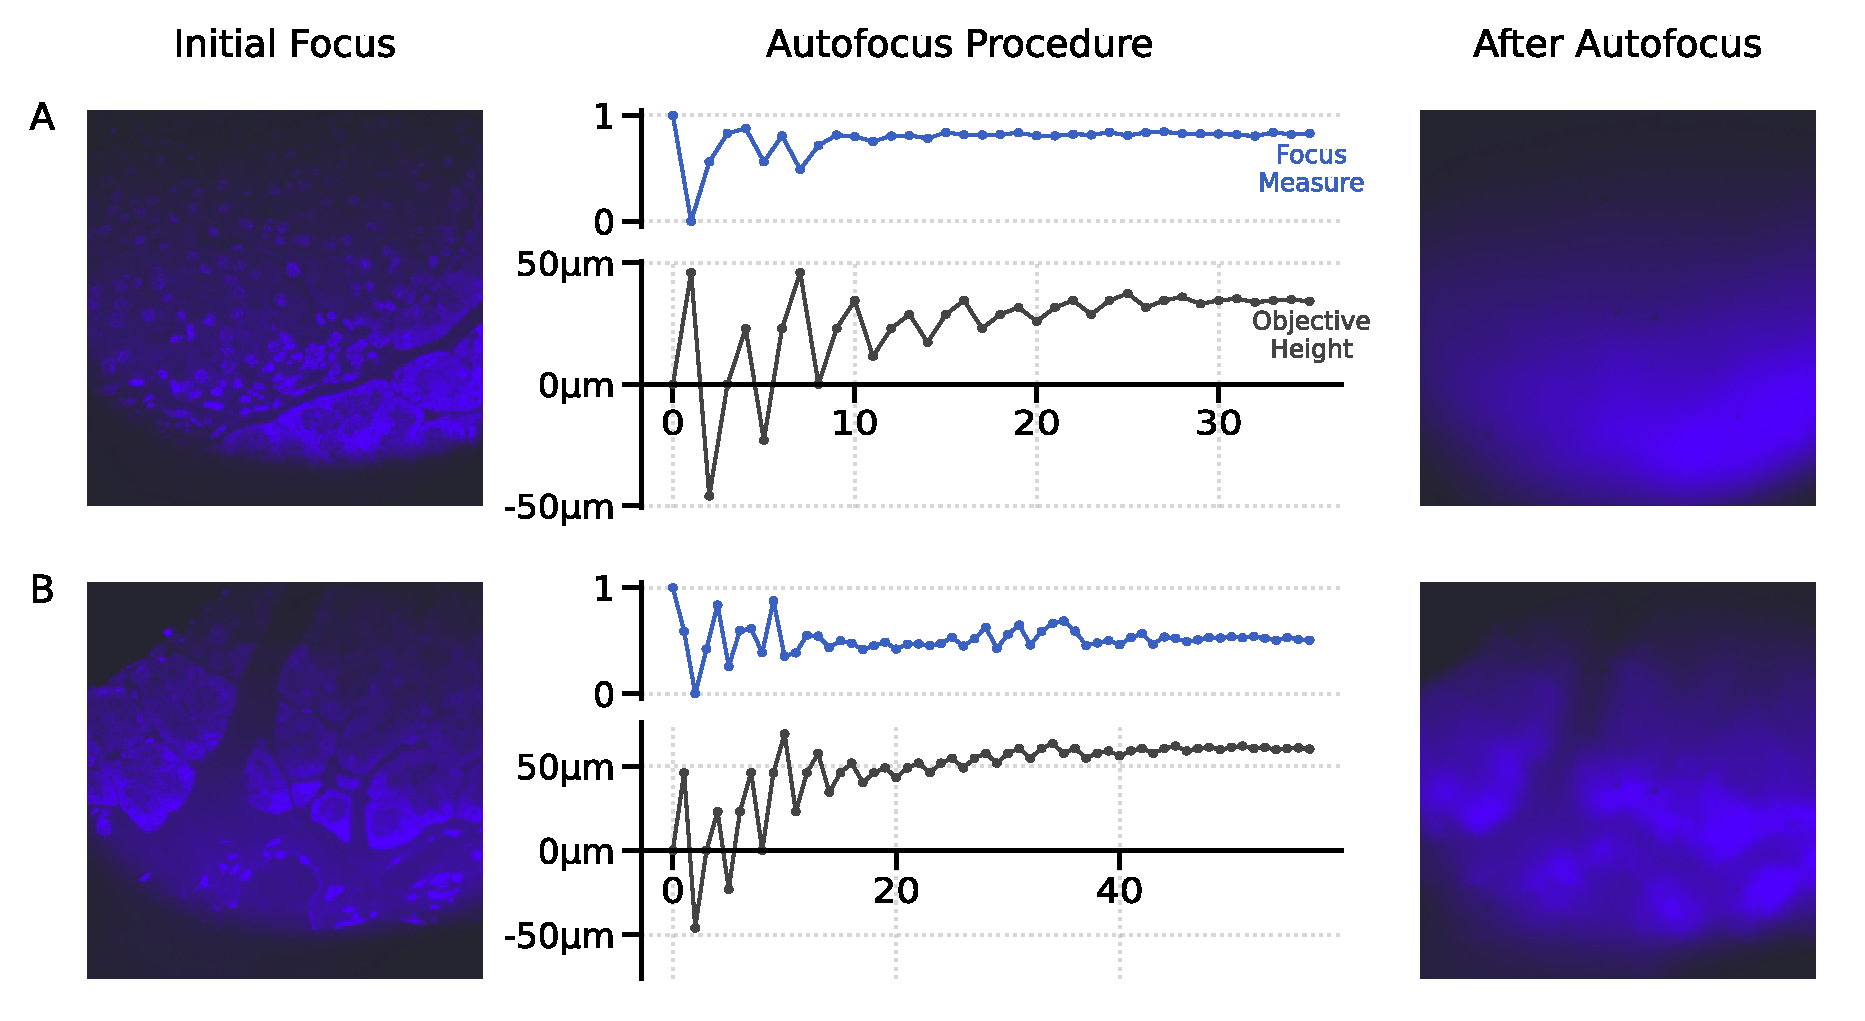
\includegraphics[width=\linewidth]{cppendix-A/figures/fig1_afruns_v3.pdf}
    \caption{Sample FM focus sweeps. x axis is iteration number}
    \label{fig:A.1_afruns}
\end{figure}


% +-----+
% | A.2 |
% +-----+
\section{Analysis of FM focus sweeps for autofocus algorithm selection}

Results in Fig A.1 / problems with autofocus suggest that the iterative nature of the autofocus routine is a possible failure mechanism as is the use of the variance of Laplacian as a focus measure. To further probe where the problem may lie / to try and possibly develop a better autofocus algorithm, we conduct a series of focus sweeps over a range of different ranges, and both fluorescence channels (Figure \ref{fig:A.2_sweeps}).

% --- Fig A.2 (sweeps) ---
\begin{figure}[!tbh]
    \centering
    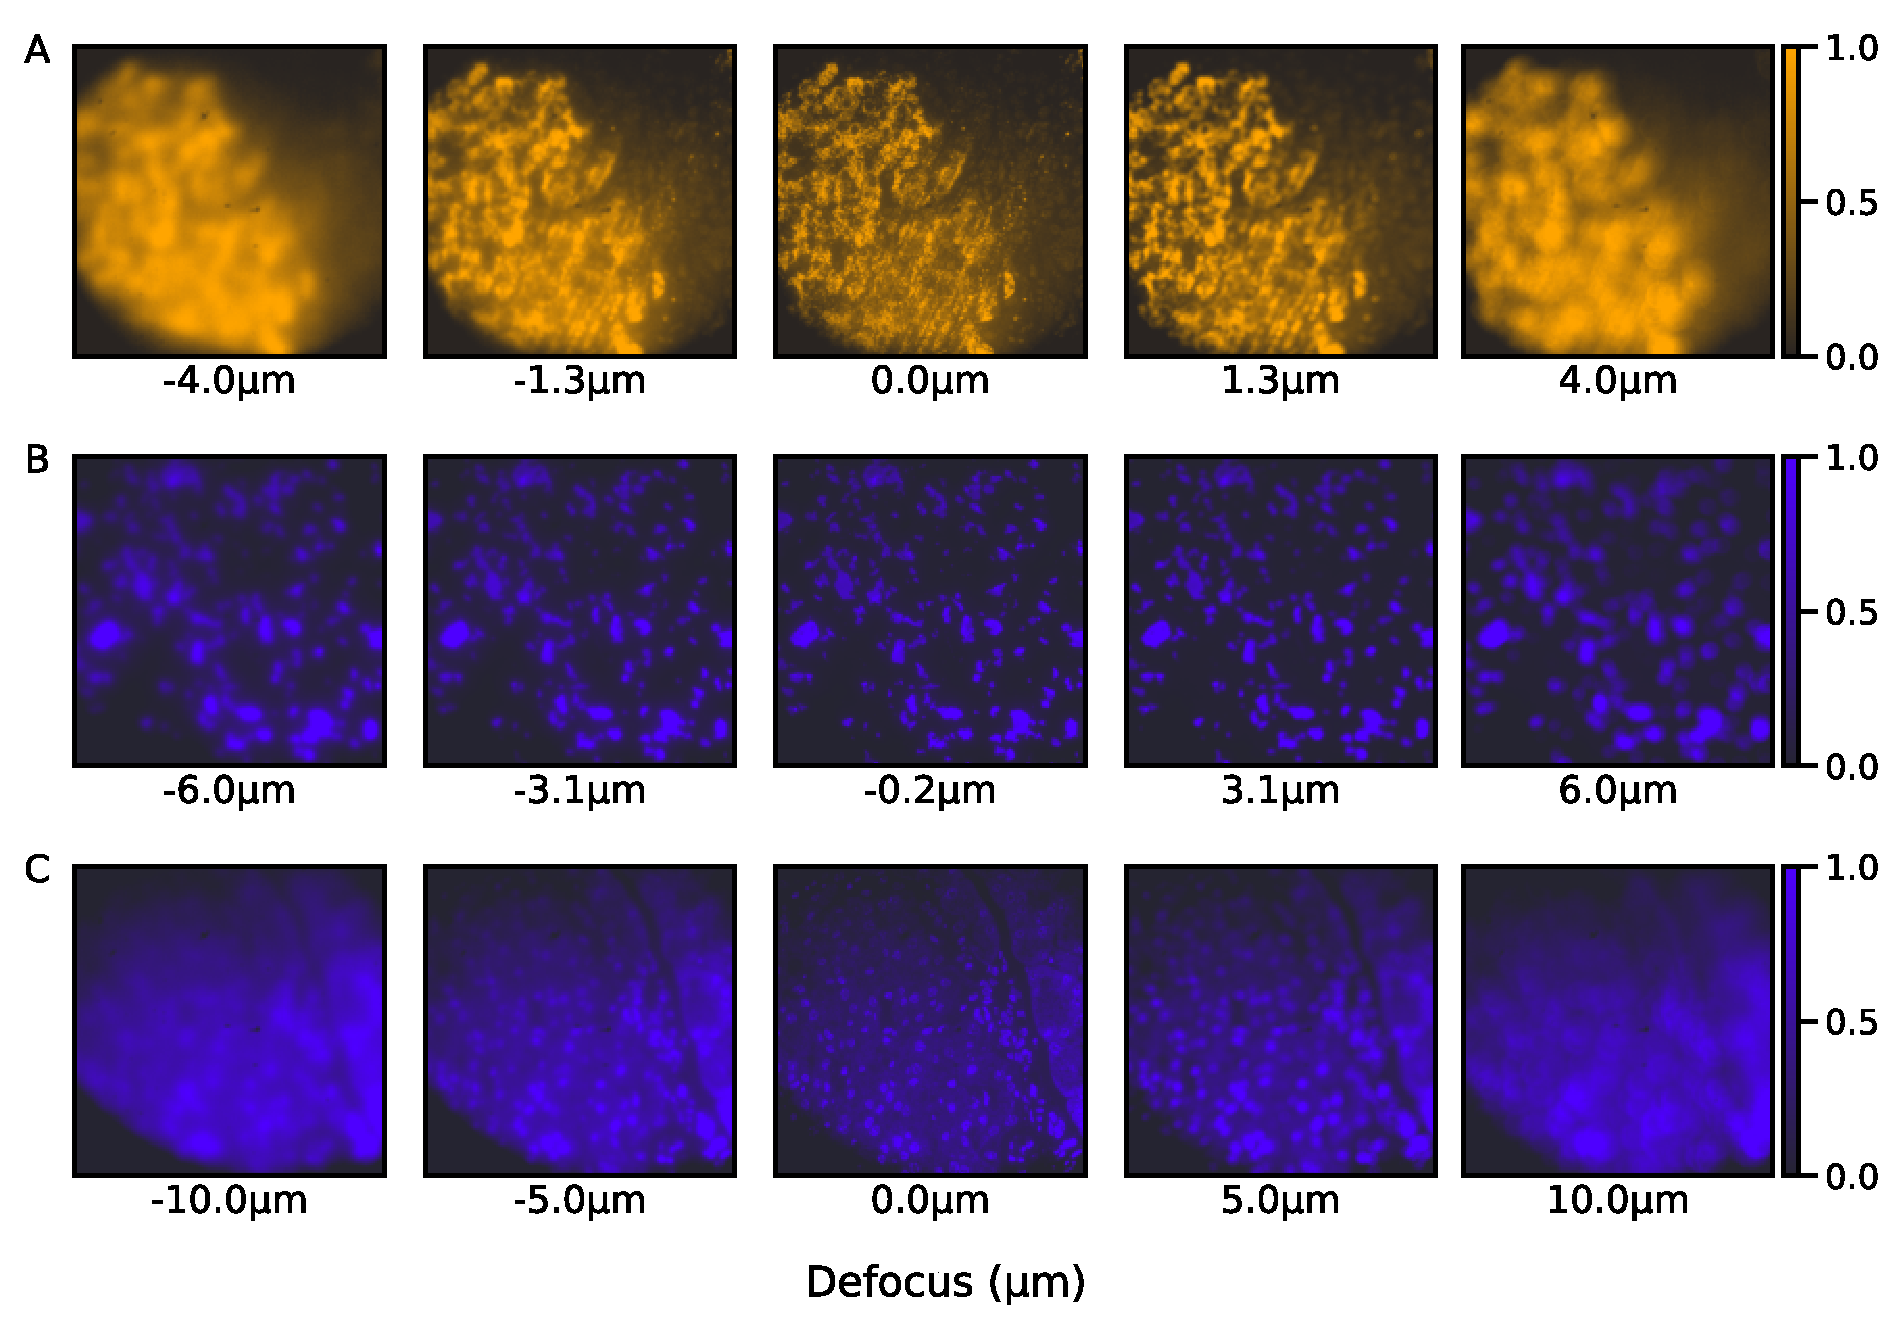
\includegraphics[width=\linewidth]{cppendix-A/figures/fig2_sweeps_v3.pdf}
    \caption{Sample FM focus sweeps.}
    \label{fig:A.2_sweeps}
\end{figure}

We then analyze the focus sweeps by applying a host of different focus measures to the data / each image in the focus sweep (Figure \ref{fig:A.3_metrics}). We get these metrics from \textcite{pertuz2013analysis}. \textcite{pertuz2013analysis} analyzed a bunch of different focus metrics to compare performance for a variety of applications. The metrics belong to different families. Explain... He concluded that "operators of the same family respond similarly to noise, contrast and window size" and that the relative performance of the focus measure operators depends highly on the imaging conditions. Here, although there is somewhat of a variety in terms of channel and scene, the imaging conditions are virtually the same. So perhaps one focus metric stands out.

% --- Fig A.3 (metrics) ---
\begin{figure}[!tbh]
    \centering
    \includegraphics[width=\linewidth]{cppendix-A/figures/fig3_metrics_v1.pdf}
    \caption{Analysis of 24 potential focus measures.}
    \label{fig:A.3_metrics}
\end{figure}

To assess the relative performance of each focus metric, we first look at how far off metrics are from picking in-focus image. This is close to 0 but not necessarily 0 because we don't want to assume that we started exactly in focus. So we take the mode from all metrics. Black means it hit peak, red means it was off with more red meaning more off. We see that Laplacian metrics have a bias towards overfocused images. We can eliminate HISE, CURV, ACMO, as well. GRAS is just GRAE (squared) and GRAT is basically identical to SFRQ for a default threshold of 0. We're not going to experiment with different threshold values as that's too much. Note that variance of Laplacian, used by Odemis, is LAPV. Now we have a number of candidate metrics. Next we can look at tougher focusing conditions and look for where methods might diverge.



 % --- Table A.1 (references) ---
\begin{table}[!tbh]
    \centering
    \caption{Reference list for focus measures.}
    \begin{tabular}{@{}llr@{}}
    \toprule
    & Focus measure & Reference \\
    \arrayrulecolor{black!30}\midrule
    \texttt{ACMO} & Absolute central moment & \cite{shirvaikar2004optimal} \\
    \texttt{BREN} & Brenner's focus measure & \cite{santos1997evaluation} \\
    \texttt{CURV} & Image curvature & \cite{helmli2001adaptive} \\
    \texttt{GDER} & Gaussian derivative & \cite{geusebroek2000robust} \\
    \texttt{GLVA} & Gray-level variance & \cite{krotkov1986range} \\
    \texttt{GLVV} & Gray-level local variance & \cite{pech2000diatom} \\
    \texttt{GRAE} & Energy of gradient & \cite{subbarao1992focusing} \\
    \texttt{GRAT} & Thresholded gradient & \cite{santos1997evaluation} \\
    \texttt{GRAS} & Squared gradient & \cite{eskicioglu1995image} \\
    \texttt{HELM} & Helmli's measure & \cite{helmli2001adaptive} \\
    \texttt{HISE} & Histogram entropy & \cite{krotkov1986range} \\
    \texttt{LAPE} & Energy of Laplacian & \cite{subbarao1992focusing} \\
    \texttt{LAPM} & Modified Laplacian & \cite{nayar1990shape} \\
    \texttt{LAPV} & Variance of Laplacian & \cite{pech2000diatom} \\
    \texttt{LAPD} & Diagonal Laplacian & \cite{thelen2008improvements}  \\
    \texttt{SFIL} & Steerable filters-based & \cite{minhas20093d} \\
    \texttt{SFRQ} & Spatial frequency & \cite{eskicioglu1995image} \\
    \texttt{TENG} & Tenegrad & \cite{krotkov1986range} \\
    \texttt{TENV} & Tenengrad variance & \cite{pech2000diatom} \\
    \texttt{VOLA} & Vollat's correlation-based & \cite{santos1997evaluation} \\
    \arrayrulecolor{black}\bottomrule
    \end{tabular}
\end{table}


% References
\printbibliography[title={References}]
 % FM autofocus


% % For format testing purposes
% \input{blindtext.tex}


% TODO:
%   Alternate (short-form) chapter titles


\end{document}
